\documentclass[9pt,conference]{IEEEtran}
\usepackage{amssymb,amsthm,amsmath,array}
\usepackage{graphicx}
\usepackage[caption=false,font=footnotesize]{subfig}
\usepackage{xspace}
\usepackage[sort&compress, numbers]{natbib}
\usepackage{stmaryrd}
\usepackage{xcolor}
\usepackage{mathtools}
\usepackage{hyperref}
\usepackage{float}
\usepackage{textcomp}
\usepackage{wrapfig}
\usepackage{titlesec}
\usepackage{multicol}
\usepackage{xcolor}
\usepackage{multirow}
\usepackage{multicol}



\titleformat{\section}
{\color{orange}\normalfont\Large\bfseries}
{\color{orange}\thesection}{1em}{}

\titleformat{\subsection}
{\color{orange}\normalfont\large\bfseries}
{\color{orange}\thesubsection}{1em}{}

\titleformat{\subsubsection}
{\color{orange}\normalfont\normalsize\bfseries}
{\color{orange}\thesubsubsection}{1em}{}

\begin{document}
\title{Developing Principled Methodologies for CNN-Based Time Series Analysis, with a Practical Demonstration using Electrocardiogram Data}
\author{\IEEEauthorblockN{
        Andrew Nash, Supervised by Prof Gregory Provan
    }
    \IEEEauthorblockA{
        BSc Data Science \& Analytics.\\
        }
}
\maketitle
\begin{abstract}

Deep learning methods have proven revolutionary in a wide range of applications from image processing, to natural language processing, speech processing and autonomous driving. Deep learning models which incorporate little to no prior domain specific knowledge can be seen to outperform the prior state of the art across many of these applications. There has been increasing research into neural networks designed to incorporate domain specific knowledge, in a similar manner to more traditional machine learning methods, which can result in improved performance. This is typically done either by use of hand-crafted input features or by defining architectures to extract features of known properties and characteristics that are traditionally associated with particular data \cite{medFeatureDNNReview} \cite{preprocessedSpeech}. Some limited efforts are being made to consider how standard models which do not incorporate domain specific knowledge might tend to converge to these domain-specific models, such as \cite{speechCNNTendstoBP}.

We demonstrate experimentally that such novel models, developed ab inito from theoretical principles, can outperform conventionally defined CNN based models. We do this using an exemplar problem (R peak extraction) on a particular class of time series data (Electrocardiogram Signals). While illustrating a novel method for R peak extraction which outperforms more conventional ResNET architectures under equivalent experimental scenarios, we validate our overall methodology and explore the applicability of our methods to other time series that exhibit the same properties as R peak extraction on ECG signals.

We conclude that this procedure of strongly incorporating theoretical properties of time series analysis into deep learning model design represents a methodology which is drastically under-valued and under-researched. The results of this research serve to illustrate only a small portion of the enormous potential of this broad methodology.

\end{abstract}

\section{Introduction}
We will restrict ourselves to the specific case of univariate time series data, a category of data with well-researched statistical characteristics, and attempt to define a general process for defining deep learning architectures that most effectively exploit these characteristics, for more robust analysis and forecasting. We will incorporate more general elements of signal processing in our analysis where appropriate - the overarching field that includes time series analysis. 

Specifically, we will focus on single-lead Electorcardigram (ECG) signals, using the MIT-BIH dataset \cite{dataset}. These signals can be considered to be variably periodic and approximately stationary time series. Components of these ECG signals and their medical interpretations are well defined in terms of duration, frequency and amplitude \cite{cardioBook}. 

Due to the prevalence of heart disease, and the significant capability of ECGs for early diagnosis of cardiac defects, automated diagnosis of ECG signals is a well-researched problem. In particular, we will focus on one of the most fundamental operations on these signals: R peak detection.

In some key aspects of ECG analysis, it can be seen that extremely simple algorithms can match, and often prove more reliable than complex deep learning models \cite{ecgReview}. Currently, some Deep Learning methods (for the most part based on CNN architectures, with some CNN-LSTM models) do achieve state-of-the art or near state-of-the art performance in QRS complex identification and ECG diagnosis. \cite{dlECGReview}. The complexities of these models are multiple orders of magnitude higher than more traditional methods, and have been shown to be more sensitive to noise. A further disadvantage of these deep models is that their internal operations are essentially opaque, making the reasoning behind a particular diagnosis in terms of some characteristics of the inputted signal.

We will consider the invariances \cite{invariants}\cite{invariantsWithDNN} associated with relevant operations required to extract R peak locations. We will form a theoretical basis for lower-complexity CNN models, that have operations with equivalent invariances and characteristics as more traditional low-complexity ECG analysis methods. Specifically, this will involve exploration of the effects applying CNN ResNET models, pooling and ReLU activation functions,  the use of bandpass filtering, Wavelet Decomposition \cite{despawn} and threshold operations.

Overall, the two main contributions of this research are:
\begin{itemize}
    \item We analyse CNN deep learning methods as applicable to time series data. We define a non-exhaustive set of pitfalls in conventional CNN architectures which lead to performance degradation for certain classes of time series inputs
    \item With a specific example of R peak extraction from ECG signals, we demonstrate the practical results of adjusting for these pitfalls, and how this can lead to more much more accurate and/or robust models compared to conventional ResNETs
\end{itemize}

We will also, in brief, consider different avenues for further development of models for different ECG diagnostic problems, with different characteristics to R peak extraction. Pursuit of this research will help develop large catalogues of CNN models that are particularly performative on very specific classes of time series data.

\section{Notation and Preliminaries}


\subsection{Time Series Modelling \& Signal Processing}
Here we state some of the most pertinent characteristics of discrete-time univariate time series data for our research. 

For general time series data, noise distributions may not be characterised using physical principles and are usually estimated statistically from the data. Most practical time-series are measured over a discrete time domain (days, weeks, months, quarters, years), particular in financial and economic applications. Time-series analysis often aims to identify the long-term trends and variations of sets of parameters. Such time-series analysis is most often used for forecasting - prediction of future behaviour. 

\subsubsection{Stationarity}
A time series is considered  \textit{strongly stationary} if its statistical properties for all continuous sub-sequences of equal size are constant. Said differently, the mean and variance of the series invariant to temporal shifts. A time series is said to be weakly stationary if the covariance between two equally sized continuous subsequences depends only on the time \textit{difference} between them, and the mean remains shift invariant. A common percursor step to modelling and forecasting a time series is to decompose the series into trend-cycle, stationary seasonal, and residual components. \cite{brockwell2002introduction} These components can be modelled independently - for example, under the Box-Jenkins framework the seasonal component can be modelled as an ARMA process.


\subsubsection{Moving Averages}
 Let $y$ be a time series comprised of $n$ observations, then a moving average of order $m$, where $m$ is odd, is obtained by
        \begin{equation}
            \hat{Y_t} = \frac{1}{m}\sum_{i = -k}^{k}y_{t+i}
        \end{equation}
        Moving averages can also be weighted - allowing more importance to be given to points closer to the point of averaging, for example. Given $a$ as a sequence of $m$ wights that sum to 1:
        \begin{equation}
            \hat{W_t} = \sum_{i = -k}^{k}a_i\,y_{t+i}
        \end{equation}
        Note that if the weights $a$ are not symmetric, the phase/time offset of the averaged series will be shifted from the original - conventionally, in time series analysis, it is customary to keep these weights symmetric as a result - as we see in \cite{brockwell2002introduction}



\subsubsection{Signal Processing}
Statistical signal processing uses the language and techniques of mathematical time-series analysis, but also introduces into the problem domain many concepts and techniques drawn from electrical engineering applications: signal to noise ratios, dynamic range, and time/frequency domain transforms.

\subsubsection{Linear Filtering}
A finite impulse response filter describes some filter in digital signal processing whose response to any finite input signal produces a finite response (one that reaches 0 in finite time). Infinite Impulse Response filters are similarly defined to not reach 0, but produce an infinite signal response for a finite input. 

\subsubsection{Convolution, Autocorrelation \& Cross-correlation}
Cross-correlation and convolution are similarly defined operations that are applied to pairs of signals, and generate single ``response" signals for each inputted pair. The sole difference between convolution and cross-correlational operations is that the convolution first flips one of the input signals along the time axis and then performs the cross-correlation. 
\begin{align*}
            CC(&p,q) = O \;\;\text{ Where}\\
            &O_x = \sum_{i=1}^{n}p_i\, q_{x+i} \\
            &\\
            CV(&p,q) = H \;\;\text{ Where}\\
            &H_x = \sum_{i=1}^{n}p_{n-i+1}\, q_{x+i}
\end{align*}

Convolution of a filter with a signal gives the output of that filter applied to the signal. Cross-correlation is used to detect whether there is a high likelihood a noisy input sequence corresponds to some known expected signal (specifically, the convolutional filter).

Autocorrelation is applied to a single signal and is the cross-correlation of this signal with itself. That has obvious use in detecting periodicity in signals and is regularly used in time series analysis for this exact purpose.


\subsubsection{Bandpass Filtering}
High pass filters, when applied to signals, attenuate low-frequency components of the signal, while allowing high-frequency components of the signal to remain undisturbed. These are commonly employed in image processing for the purposes of image sharpening, and edge detection. They are not particularly robust at detrending data, and thus should not be used for that purpose. Low pass filters work similarly to high pass filters, boosting low frequencies, but not high frequencies. This is typically useful as a form of denoising or local averaging. Band pass filters combine both high and low pass filters, to remove frequency components above or below a certain thresholds from a signal.

\subsubsection{Matched Filtering}
The purposed of applying a matched filter is to identify the presence of known wavelets in a potentially noisy input sequence. This is obviously of particular use in radar and sonar signal processing. The optimal (maximised Signal-to-Noise Ratio) filter for detecting a particular wavelet is the time reversed wavelet, with which the input signal is cross correlated \cite{bancroft2002introduction}.

\subsubsection{Wavelet Decomposition}

We previously mention the commonality of processing and analysing digital signals in the frequency rather than the time domain. There are a few methods by which this is achieved, such as the Fourier Transform, Short-Term Fourier Transform, Hilbert-Huang Transform and Wavelet Decomposition. The wavelet decomposition is of particular importance for ECG analysis.

The aim of wavelet analysis is to overcome the time-frequency uncertainty principle of the FT/STFT. Given some fixed, predefined wavelet signals, these are scaled and stretched by different amounts, and each convolved with an input signal. Doing this allows information the presence of known signals within the unknown signal allows us to identify information about the instantaneous frequency of the signal at all points in time, without a loss of frequency resolution.

\subsection{Invariants}
 All time series can be characterised by a number of different properties - overall mean, (or mean amplitude for periodic data), trend, period of seasonality, overall duration, etc. Many operations we perform do not need to take all of these characteristics into account. In the case of ARMA models, operating under the assumption of stationarity, the absolute temporal information of observed values are ignored, allowing us to consider \textit{relative} temporal differences only. This disregarding of certain time series properties is the principle of invariance. Based on \cite{batista2014cid}, the following are definitions of most classes of invariance applicable to time series.
\subsubsection{Amplitude \& Offset Invariance} An operation is amplitude invariant on two signals if it generates the same output regardless of scalar multiplication of either of the signals by a (strictly positive) constant. Offset invariance is similarly defined, allowing addition of any scalar constant value to either of the signals.
\subsubsection{Local Scaling/Warping Invariance} An operation is local-scaling invariant if outputs are consistent in the presence of small local accelerations and decelerations (expansions and contractions) in time take place in each of the input signals. This is particularly important when modelling physical and biological systems. 
\subsubsection{Uniform Scaling} Uniform scaling invariance is similar to local scaling invariance - but refers to the entirety of one signal being accelerated or decelerated relative to the other. This is generally difficult to account for by any means other than exhaustively testing possible values.
\subsubsection{Shift/Phase/Temporal Invariance} Phase invariance is achieved when phase differences (offests in time) between the inputs does not change the result.
\subsubsection{Occlusion Invariance} Occlusion invariance is achieved when operations return the same (or, in a more realistic scenario, close to the same) result when small segments of the input signals are missing.
\subsubsection{Complexity Invariance} Proposed in \cite{batista2014cid}, complexity invariance refers to operations that generate the same results on input signals that share some underlying patterns, but at different levels of resolution or frequency.



\subsection{ECG Analysis}
Before considering computational methods for analysing ECG signals, we will first review the physiological characteristics described by ECG signals.

ECG waveforms corresponding to a single heartbeat (Fig \ref{fig:ecg_components}) can be split into the following wavelets \cite{cardioBook}.

\begin{enumerate}
    \item P wave. This corresponds to atrial depolarization (contraction) 
    \item QRS complex. Small Q waves correspond to depolarization of interventricular septum, and can be affected by breathing. If they are big, can correspond to an anomaly (such as myocardial infarction - i.e. blood clot). The R wave corresponds to depolarization of the main mass of the ventricles. S wave corresponds to final depolarization of the ventricles at the base of the heart.
    \item The T wave represents ventricular repolarization
    \item U waves, which are of unknown source, and low in amplitude
\end{enumerate}

\begin{figure}[H]
\centering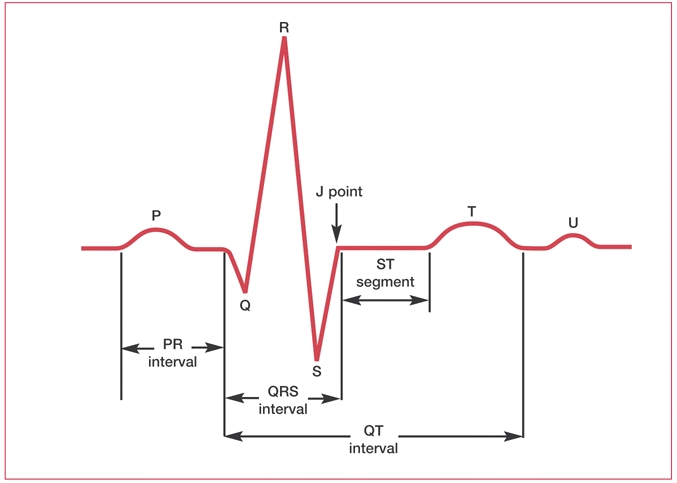
\includegraphics[width = 0.35\textwidth]{ecg_components.jpg}
\caption{\label{fig:ecg_components} Components of an ECG waveform}
\end{figure}

Typically, when looking at an ECG, clinicians will take the following characteristics into account:

\begin{enumerate}
    \item[\textbf{Rate}] The intervals between QRS complexes are an indicator of heart-rate.
    \item[\textbf{Rhythm}] The morphology of the different components, and the intervals between them can indicate any deviation from the expected/healthy sequence of operations. For example, and absence of P waves and irregular and narrow QRS complexes are one indicator for atrial fibrillation.
    \item[\textbf{Axis}] Only applicable to multi-lead ECGs, this is a determination of the direction of electrical activity around the heart. It is determined comparing the differences in amplitude between the R and S waves on different leads.
\end{enumerate}

Deviation from the defined well-known expectations of the above values can be indicative of specific cardiac abnormalities \cite{cardioBook}.

\subsection{Automated ECG Diagnosis}
Automated ECG Analysis has been extremely widely researched over the last number of decades for a range of clinical applications. We will consider a single lead ECG, generating a univariate time series. The main clinical application of single lead ECGs is in small form-factor long term cardiac monitoring devices that generate very long signals which cannot feasibly be diagnosed by hand.

\subsection{ECG Signals as Univariate Time Series}
The following time series properties are exhibited by ECG signals:

\paragraph{Stationarity \& Homoskedasticity}
ECG signals cannot be assumed to be stationary in realistic conditions. Baseline wander is observed due to external electrical interference, as well as other biological factors such as respiratory and muscular activity. In the case of baseline adjusted signals, the mean can be assumed to be stationary, with minor variations. In neither case can the variance be assumed to be constant - the rate and rhythm of the cardiac activity will vary over the course of the ECG, and this may or may not have diagnostic significance.

\paragraph{Periodicity}
The ECG waveforms themselves are not seasonal but variably periodic, where the implicit time series of periodicity changes is of clinical significance.


\paragraph{Shift Invariance}
As a consequence of these properties, shift invariance does not strictly apply to ECG data. Any shift invariant methods that are applied must be sufficiently robust to variations in the periodicity/heart-rate, and be applied in a windowed manner over a sufficient duration of the time series to be able to capture localised variations in the waveform periodicity.

\paragraph{Amplitude Invariance}
Due to factors such as the natural differences between patients, the placement of ECG leads, the accuracy of the ECG monitoring device, and the degree of noise present there is some minor variation in the voltage measured of adjacent waveforms. In some cases this may be indicative of a clinical or experimental anomaly. In the general case, any analysis should be robust to these amplitude variations.

\subsubsection{QRS Complex Detection \& R Peak Extraction}

Since the QRS wavelet is the dominant repeating component of an ECG signal, it makes sense to identify the locations of these complexes as the first step of any automated signal diagnosis pipeline. \cite{ecgReview} provides a good review of current methods used to perform computational QRS complex detection.

The most common techniques for performing QRS complex detection can be broadly separated into two classes:

\begin{enumerate}
    \item \textbf{Signal Processing Techniques}, particularly the use of bandpass filtering and wavelet decomposition.
    \item \textbf{Deep Learning Models} of many varieties have been applied to different levels of success, but have not generally achieved the revolutionary level of performance as many other application domains
\end{enumerate}

This is not an exhaustive classification of diagnostic methodologies, but covers the most important and well-applied, and are thus what we will focus on.

We will consider both of these methodologies, assessing their capabilities on time ECG time series based on how properties such as stationarity, variable periodicity, and requirements for shift and amplitude invariances are handled by each.

\subsection{Deep Learning for Time Series Analysis}
The unreasonable success of Deep Learning models across an enormous variety of application domains - including many instances of time series analysis and forecasting.

Some of the most commonly applied deep architectures for time series data, as per a recent review \cite{dlTSReview}, are:
\subsubsection{Deep feed forward neural network}
The most traditional method of architecting a deep model, involving consecutive layers of composed non-linear functions of weighted combinations of previous layers' outputs. 

\begin{equation*}
    a^l = g\left(W_a^la^{l-1}+b_a^l\right)
\end{equation*}

Where $a^l$ is the output of the $l$\textsuperscript{th} layer of the model, $W$ and $b$ correspond to learnable weight and bias parameters, and $g$ is a non-linear (usually monotonic) function such as Sigmoid or a Rectified-Linear Unit (ReLU).

This architecture has no particular specificity to time series data, so we largely disregard it in this research.

\subsection{Convolutional Neural Networks}
These models can be considered to simply learn \textit{cross-correlational} filters (also known as kernels) (for easier numerical computation than a true convolutional filter) in place of the $W$ matrix defined for a standard DNN.

These has demonstrated excellent performance in particular in image processing, as well as in time series applications such as \cite{stanfordML}.

A modification of these networks known as the Temporal CNN has become increasingly popular in recent years. While standard CNN models typically involve downsampling of signals between layers by pooling - most often max pooling - TCNNs instead \textit{dilate} the filter sizes at each layer.

Where a standard CNN kernel application can be evaluated as the $CC$ function in Section II-C1 above, a dilated CNN is applied in a manner more closely resembling:

\begin{align*}
            CC(&p,K) = O \;\;\text{ Where}\\
            &O_x = \sum_{i=1}^{n}p_i\, K_{x+\left(i\times d\right)} \\
\end{align*}

Where $d$ is a parameter that controls the extent of the dilation on the CNN kernel $K$. These have been generally praised for their benefit of improving the \textit{receptive field} \cite{wang2017dilated} of the layers. We will show that this is not actually telling the full story for certain classes of time series, and that dilations allow CNN models to comply more reliably with shift invariance. 

\subsubsection{Recurrent Neural Networks}
One of the earliest introduced time-series specific architecture, these models are recurrent structures, where the outputted prediction of internal state variables are recycled as inputs to the same internal state variables in a recurrent \textit{cell}.

Specific RNN architectures, particularly Long short-term memory models have shown better performance over more trivial RNN implementations. Nonetheless, these models tend to often encounter issues with vanishing gradients and are theoretically challenging to formally analyse. For this reason, we will not be addressing their use and development in this research. We will consider the state-of-the art model defined in \cite{stanfordML}, which consisted of a standard 1-D Convolutional ResNET implementation.


\subsubsection{Residual Neural Network (ResNET)}
ResNETs\cite{he2016deep} are relatively simple modifications of other (typically CNN) architectures, where some of the connections between layers will \textit{skip} forward multiple layers in the network. This leads to better training, conventionally attributed to better robustness to vanishing gradients, allowing much deeper models to be effectively fitted.




\section{Existing methodology for ECG analysis}

\subsection{Mathematically Modelling \& Characterising an ECG Signal}
Before performing any automated diagnosis of ECG signals we must first create some mathematical representation in which to express them. Over the many years of ECG research, experimentation across a multitude of different approaches has lead to the identification of some notably successful models for ECG analysis.

\subsubsection{Combination of multiple statistical processes}
There have been some attempts to model ECG signals as well defined compositions of precisely defined processes. \cite{Napolitano2022Jan} attempts to form a very precise expression for a healthy ECG signal as an explicitly defined statistical processes. This appears to have been at least in part inspired by \cite{coupledECG} which modelled ECG signals as coupled systems of ordinary differential equations. Other similar approaches are referenced in the introduction of \cite{Napolitano2022Jan}.

\subsubsection{Combination of multiple reference wavelets}
Other approaches \cite{shapeMatch2007} attempt to build a library of known wavelets within ECG signals that correspond to certain clinical diagnoses. Such models use distance measures such as DTW to determine the most relevant known wavelets (with known clinical dignoses) to an undiagnosed signals. 

\subsubsection{Drawbacks of an explicit mathematical model or statistical process}
While being able to describe ECG signals as composition of known statistical processes would be extremely desirable, this approach has not been widely adopted (to the best of our knowledge) and is generally overlooked in recent research. 

The first reason is the large degree of noise present in ECG signals from a variety of different sources.

 \cite{Napolitano2022Jan} states they the are working under the assumption of additive noise that is independent of the ECG signal. However, \cite{ecgNoiseReview} describes some of the most common sources of noise in ECG signals - namely baseline wander, power-line interference, and muscle artefacts. As a simple violation of the independence assumption, we can expect higher levels of muscle artefacts and baseline wander where increased levels of respiration and movement are observed in patients with an elevated heart rate. This results in noise that is correlated to the RR intervals of the patients' ECG signals. 

 Secondly, there is a huge amount of natural variability between healthy ECG signals for different individuals. In \cite{ecgPractice} we see that S waves can sometimes be greater in amplitude than R waves in lead 1 of 12 lead ECGs (commonly used for single lead ECGs). We also see that abnormal P waves are not indicative necessarily of cardiac defects if observed as part of  a `ectopic atrial rhythm`.

The placement of the leads will determine the axis of observation, and thus differences in placement of the leads between patients will result in small relative differences between the strength of different components of the ECG signals between patients, or indeed for different recording sessions for the same patient.

Ultimately this leads to a highly coupled system of enormous complexity. There are an enormous number of potential transformations of the basic components of an ECG, whose interpretations are all strongly interlinked. Manual codification of these in a manner that is robust to uncontrollable external sources of noise is an unreasonably difficult challenge.

\subsection{Statistical Feature Extraction \& Classification Methods}
A variety methods have been proposed to identify the locations of QRS complexes, by the classification of different sets of features, broadly categorised in \cite{Gupta2021Oct} as:

\subsubsection{Feature Extraction}
\paragraph{\textbf{Time domain features}}
Morphological features of the ECG considered in the time domain. This can often involve the application of matched filters, where distance metrics such as Dynamic Time Warping (DTW) are computed to known reference templates to act as the primary features for classification. Other models utilise the measurements of the intervals between positive matches from such templates as classification features.

\paragraph{\textbf{Frequency domain features}}
These methods focus on measuring the concentration of power in different frequencies in the Fourier Transform (or Power Spectrum) of the signal.

\paragraph{\textbf{Time-Frequency domain features}}
As a compromise between the above, these methods attempt to extract features that are compromises between the capabilities of the two feature sets. Methods such as STFT, Hilbert-Huang transform and Wavelet analysis are used to accomplish this. Across the literature, wavelet transforms appear to be by far the most commonly applied to ECG signals of these different methods.

In a slightly more clinically-oriented framework, \cite{KAPLANBERKAYA2018216} attempts to describe more a different set of features that can be extracted from raw signals for classification:

\paragraph*{a) \textbf{P-QRS-T complex features}}
A subset of the class of time domain features, this category has the added restriction of features that are based on some morphological relationship between an unknown signal (or portion thereof) to a known signal representative of some \textit{known characteristic} of a reference ECG signal.

This therefore involves the use of some processing methods to identify likely Q,R,S and T peaks in an undiagnosed ECG, to generate these higher level features.
\paragraph*{b) \textbf{Statistical features}}
This refers to basic summary statistics that can be calculated on any time series - mean, standard deviation, minima and maxima, etc.

\paragraph*{c) \textbf{Morphological features}}
Distinct from P-QRS-T complex features, these are a specific set of time domain features with no underlying reference to some ground-truth clinical component of a general ECG signal. For example, \cite{polyApprox} use polynomial approximations of ECG signals as features for a diagnostic model.

\paragraph*{d) \textbf{Wavelet features}}
Due to the ubiquity of wavelet transforms in ECG diagnosis, the review overlooks features purely in the frequency domain (such as the Fourier Transform), and does not consider other time-frequency representations, such as the STFT or Hilbert-Huang Transform, only considering the wavelet decomposition.

\subsubsection{Identification of QRS Complexes By Signal Processing Techniques}

\cite{ecgReview} provides a review of these methods applied to the specific problem of QRS complex detection. Many of the methods applied consist of two distinct stages: preprocessing and  classification/detection.

\paragraph*{a) \textbf{Signal Pre-processing methods}}
\begin{enumerate}
    \item Band-pass filtering
    \item Wavelet Transform
    \item Empirical mode decomposition
    \item Derivative Filtering
    \item Moving Average Filtering
\end{enumerate}

\paragraph*{b) \textbf{Detection methods}}
\begin{enumerate}
    \item Thresholding on the pre-processed signal. It is noteworthy that some of the more successful methods implemented \textit{adaptive} thresholds \cite{adaptThresh}, where a pre-defined upper and lower threshold are iteratively reduced and increased respectively until correspondence is achieved
    \item Moving Average Filtering
    \item Zero Crossing detection on the pre-processed data. This is particularly relevant when applied to derivative filters, and when used with wavelet transformations, due to the large gradient changed on the RS and QR intervals.
    \item Singularity point detection - similar in practice to Zero Crossings on wavelet transforms, singular points are those which have derivatives of opposite signs to the left and right \cite{singularECG}  
\end{enumerate}


\subsubsection{Identification of QRS Complexes By More Complex Modelling}
In an attempt to reduce the amount of required manual pre-processing and achieve more accurate predictions, there is extensive literature \cite{ecgReview}\cite{KAPLANBERKAYA2018216} that attempt to fit complex models both to some of the pre-processed features listed above, and also to raw ECG signals.

Examples of such methods are:
\begin{enumerate}
    \item Neural Networks applied to the raw signal
    \item Hidden Markov Models applied to the pre-processed signal
    \item Syntactic pattern recognition on the raw data. This is similar to HMM models, and the previously mentioned methods to explicitly model the different components of ECG signals
    \item Bayesian Classifiers
    \item Support Vector Machines
\end{enumerate}

While neural networks are most commonly applied of these these models, it has been noted that the Neural Network models were particularly noise sensitive.

Studies, such as \cite{dogan_dogan_2023} (published only a week before the time of writing), consistently indicate that the most advanced neural network models with much higher levels of computational complexity, achieve at-best marginal improvements over well established filter-and-threshold based signal processing methods for QRS complex detection.

\subsection{Contrasting Wavelet based and CNN based methodologies}
It is interesting to note the extent to which neural network models have struggled to match the performance of extremely low-complexity models, while retaining a higher degree of noise sensitivity.

It is immediately noticeable that CNN models and wavelet decompositions have some striking structural similarities.

Most wavelet decompositions consist of multiple levels of high-pass filters followed by decimation of the outputs (usually by a factor of 2, for a so-called \textit{Dyadic} wavelet decomposition). This is followed by thresholding on each level of the \textit{coefficients}, and finally recomposition of all the coefficients by low-pass filters and up-sampling.

These filters are computed analogously to the kernel convolution computations in CNN models. The architecture of a wavelet decomposition is therefore very similar to that of a CNN auto-encoder, with modified residual connections. Indeed, there have been some wavelet based CNNs that are specifically designed to even more closely resemble wavelet transforms, such as \cite{despawn}.

Even with these structural similarities, CNN models require vastly higher complexity to reach similar levels of performance, and even then, at lower levels of robustness in the specific case of R peak extraction. Therefore, there is at least one aspect of the simple wavelet \& threshold model that CNN models struggle to capture - either the capability of the wavelet transform to accomplish effective feature extraction, its capability to learn an effective decision boundary on the extracted features, or its capability to perform both jointly.

\section{General Characteristics of R Peak Extraction}
In order to assess the general capabilities of these differing approaches, we will consider the general problem of R peak extraction, as pertains to an abstract time series. The characterisation of an ECG as a general time series is already described in our preliminaries.

We can consider ECG signals as having approximately constant mean, variable periodicity, variable amplitude across periods, and exhibiting highly complex non-stationary noise that has a trend, cycle, and may be partially correlated to some clinical properties of the signal. The most important aspect of this is the noise, which is challenging to deal with.

R peak extraction can be considered on such a general series to be the process of isolating the positions of the highest amplitude component of the variably periodic wavelets of the signal. Take note that this may not be the actually observed highest amplitude component of an observed signal, and further, the highest amplitude component of an observed signal may not correspond to a true peak. Our definition of a peak, is that of the true maximum, generated by some characteristic of the underlying process of the time series, that can be observed in a perfectly noiseless signal. Obviously, even the best prediction model will generate false detections in the presence of sufficiently strong noise.

Such a model should output a sequence of 0/1 values corresponding purely to presence/non-presence of this component at a given time point in the signal - this output should be of uniform amplitude. In the case of R peak extraction, wavelet models often explicitly incorporate prior knowledge about expected intervals on these predictions, and it is assumed that neural network models will implicitly learn these distributions. However, we will drop this component from our general model, to allow for broader conclusions. Henceforth, we will refer to this generalised problem as peak amplitude detection, to create a distinction from the specific instance of R peak extraction. 

\subsection{Peak Amplitude Detection}

The ideal peak amplitude detector, which perfectly identifies peak amplitudes for all possible input signals observes the following invariances, at a minimum:

\paragraph{Conditional Amplitude Invariance}
The restriction of the model to purely positional information (1/0) outputs is in fact a form of conditional amplitude invariance. The detector must effectively create two sets of decision spaces, where an observation, or set of observations, falls into one set or the other, corresponding to peak amplitudes or non-peak amplitudes. The model is obviously, by design, invariant to local variations between observations in the same set. An example of this can be seen with models based on thresholds - the threshold creates a decision boundary that delineates the sets of peak and non-peak amplitude observations. Said differently, the threshold operation is invariant to variations in amplitude that do not cross the decision boundary - i.e., it is conditionally amplitude invariant.

\paragraph{Shift Invariance}
The operation of peak amplitude detection must clearly be shift invariant - a peak should be detected regardless of the overall phase of the input data.

If a method does not exhibit these characteristics, it will not be \textit{robust} to irrelevant variation input data, no matter its level of complexity or degree of optimisation. This problem should also incorporate Local Scale, Uniform Scale, Complexity invariance, but these will not be as important in the following discussions.

\section{ Inherent limitations of deep-learning for ECG analysis: First-principles methodology}


\subsection{Assessing the behaviour of wavelet decomposition on Shift Invariant data}

By the mechanism of the convolutional/cross-correlational operations that are equivalent across wavelet and CNN models, it is easy to see that these operations appear to be shift invariant. However, in fact, downsampling in both approaches will result in violation of shift invariance.

Downsampling in traditional signals processing is typically performed by taking the average over consecutive disjoint sets of values, to correspond to a single value in the downsampled signal. E.g., pairs of adjacent values can be averaged to correspond to a downsampled signal of half the length of the input.

In the case of wavelet transforms, the low pass filter has an anti-aliasing affect, which mitigates the effect of the shift variance of the downsampling operation. \cite{bradley2003shift} However, with increased thresholding, this breaks down, allowing variations caused by constant shifts to creep in. A modified wavelet transform, the \textit{algorithme à trous}, can achieve shift invariance with equivalent predictions. It does this by expanding (dilating) the filters by 0 padding between filter element at each level instead of directly downsampling the signal.

\subsection{Assessing the behaviour of CNN models on Shift Invariant data}
Similarly, for CNN models, the pooling operation is not shift invariant. However, there is a modification of CNN models to achieve better shift invariance known as a dilated CNN, which are analogous to the algorithme à trous in terms of dilating the kernels rather than downsampling the input data.

Therefore, for a general truly shift invariant operation, particularly such as in this instance, where we wish to precisely locate a feature to within a single sample, these dilated filter operations are much preferable.

\subsection{Assessing Wavelet and CNN model behaviour on Conditionally Amplitude Invariant data}

The conditional amplitude invariance is achieved trivially with hard thresholds in the wavelet decomposition models - where the construction of the 1/0 outputs is explicitly coded into such models. However, there are two slightly different types of conditional amplitude invariance achieved, depending on whether the thresholds are pre-defined as specific amplitude values, or relative - where the thresholds are computed as a certain percentile of the observations. Adaptive thresholds are a slight modification of relative thresholds, where independent thresholds are computed over subsections of the data.

\paragraph{Global Thresholds}
For a fixed, pre-defined threshold, the outputs are invariant to variations in the inputs that do not cross the threshold. Said different, it is invariant to localised variations on either side of the decision boundary.
\paragraph{Relative \& Adaptive Relative Thresholds}
For a relative threshold, the outputs are amplitude invariant - multiplying the entire signal by a constant factor will not affect results. It also demonstrates the same conditional invariance as global thresholds, where the outputs are invariant to variations within the lower and upper percentiles that do not alter the computed threshold position.

\subsection{Assessing CNN Model behaviour on Conditionally Amplitude Invariant data}

The main mechanism by which a CNN model can form a decision boundary for 1/0 classification, from some arbitrary weighed output, is by use of non-linear activation functions. Here, we will first consider which properties of an ideal peak amplitude detection model are exhibited by an individual activation function. Then, we will generalise this to compositions of activation functions to better reflect a full deep model.

\paragraph{Activation Function Properties}
Traditionally, many activation functions used in neural network models, such as tanh and sigmoid activation functions closely resemble soft-threshold functions. The Heaveside step function, or true threshold, has long been proposed for different deep models, but rarely applied to due the impossibility of training by gradient descent.

It can be easily shown that any activation function that has bounded outputs will experience vanishing gradients in the upper and lower limits.

Let  $f\left(x\right)$ be an arbitrary monotonic function. We will not consider activation functions that are not monotonic in the limit, as these have no practical benefits. Let us assume $f$ is monotonically increasing, with domain $\left[a,b\right]$.

\begin{equation*}
 \implies \lim\limits_{x\to -\infty} f\left(x\right) = a, \lim\limits_{x\to \infty} f\left(x\right) = b 
\end{equation*}

Using Newton's Quotient as an estimate of the derivative of $f$:

\begin{equation*}
f^\prime\left(x\right) = \lim\limits_{h\to 0}\frac{f\left(x+h\right)-f\left(x\right)}{h}
\end{equation*}

However, under the limit $x \to \infty, \left|f\left(x\right)-f\left(x+\delta\right)\right|=0$, by construction of $f$
\begin{equation*}
    \implies f^\prime\left(x\right) \approx \lim\limits_{h\to 0}\frac{f\left(x\right)-f\left(x\right)}{h} = 0 \text{ as }  x\to \infty
\end{equation*}

Clearly, any fully bounded function has a 0 derivative in the upper and lower limits - causing a vanishing gradient that kills optimisation.

Further, as the activation approaches a perfect decision boundary, with outputs that approach perfect segmentation into exact $a$ and $b$ values for all values of $x$, the gradients approach 0. This is a straightforward consequence of the well known vanishing gradient problem.

A common approach to address vanishing gradients in activation functions such as ReLU is to remove the bounds on the function, and enforce a lower limit on the gradient of the function. It is easy to intuit, and demonstrate, that the higher the lower bound on the gradient, the more the bounds on the original function are violated

Here, we will assume that $f\left(x\right)$ crosses the x-axis at (0,0) without loss of generality

Assume that, in order to address the vanishing gradients of $f$ previously demonstrated, we impose a lower bound on the gradient of $f$ - $\text{min } f^\prime\left(x\right)=\delta_\text{min} \; \forall x\; \in\left[0,\infty\right]$

Considering  $\;f$ on $x\;\in\;\left[0,\infty\right]$, monotonically increasing, a lower bound on $f\left(x\right)$ is 

\begin{equation*}
f\left(x\right)=\int_0^x\delta_{\text{min}}\text{dx}=x\delta_{\text{min}}
\end{equation*}

In the best case, the bounds on $f$ therefore increase linearly in magnitude with the inputs.

We can thus further elaborate on our tradeoff - as the gradient-based trainability of a particular function increases, its ability to define a true decision boundary (at best linearly) decreases.

\paragraph{Activation Function Trainability/Bounding Tradeoff}
As a consequence, there is a fundamental inability for an activation function's ability to form a conditionally amplitude independent binary classification threshold.

If such a threshold exists, with outputs that are equal to some upper bound and lower bound value, this activation function must have a 0 gradient, making it untrainable by gradient-based optimisation.

Here, we define gradient-based optimisation as any optimisation method which uses any objective function that consists of some multiple of the activation function's gradient $f^\prime\left(x\right)$.

Trainability of these activation functions is only possible when:

\begin{enumerate}
    \item The outputs of the activation functions are distributed between $a$ and $b$, at a significant distance from the upper and lower limits. 
    \item The activation function is unbounded
\end{enumerate}

In both cases, we are in violation of the conditional amplitude invariance, as local variations within each decision set (above and below the decision boundary), generate different outputs. 

\paragraph{Generalisation to a multi-layer network}

Thus far, we have only considered the case of a single activation function. The situation is slightly different when considering a multi-layer network, but we will see that similar properties hold.

Let us consider the case where the bounded decision-boundary classification function $f(x)$ is composed of multiple non-linear functions which may not necessarily individually have vanishing gradients on different intervals, $f(x)=g\circ h(x)$.

Letting $y = g\circ h(x) = g(h(x))$, assume $\displaystyle \frac{\delta y}{\delta g}$ does not necessarily have a vanishing gradient. 

\begin{equation*}
\displaystyle \frac{\delta y}{\delta x} =  \frac{\delta y}{\delta g(h(x))} \times \frac{\delta g(h(x))}{\delta h(x)} \times  \frac{\delta h(x)}{\delta x} = f^\prime(x)
\end{equation*}

$f^\prime(x)$ by the above argument, will still experience vanishing gradient if it is capable of representing a conditionally amplitude invariant decision boundary. If we consider this to correspond to a multi-layer neural network of two layers ($h$ and $g$), applied to inputs $x$, we see that the vanishing gradient $f^\prime(x)\to 0$ occurs once we backpropogate to the input layer. In this case, such the weights of the lower layer ($g$) will be trainable, but the upper layer $h$ will likely not. 

Now consider the case of a hypothetical complex multi-layer network of $>2$ layers, which has a number of pre-processing layers that output some tensor $x$, which acts as input to layer $h$. If $g\circ h$ defines a conditionally amplitude invariant threshold boundary, this will clearly annihilate the trainability of the prior pre-processing layers, restricting the trainability of the overall model.

As an overall consequence, the more accurately any neural network model becomes at forming a true decision boundary that is robustly invariant to noise above and below the boundary, the less trainable this network will become.

\paragraph{Batch Normalisation}
A extremely prevalent method to address vanishing gradients in deep models is the use of normalisation. This is typically applied over batches, although weight and layer normalisation have also been proposed and applied in some instances.

\cite{invariantsWithDNN} (a rare piece of research into deep models that respect time series properties) notes that normalisation is not always appropriate for time series modelling for deep learning. This is due to the lack of a known supremum and infimum for a general time series, and lack of stationarity. 

Here we will consider the case of an approximately stationary time series, where batches consist of adjacent or overlapping windows of observations for maximal consistency within batches. We will also assume that outlying extrema are either not present, or extremely rare in the series.

In this instance, we will consider what improvement, if any, will normalisation lend to the aforementioned issues with trainable and robust decision boundaries.

Batch normalisation, as defined in \cite{invariantsWithDNN}, is
\begin{equation*}
    \mu_B = \frac{1}{m}\sum_{i \in \left[1,m\right]}x_i, \sigma_B^2 = \frac{1}{m}\sum_{i \in \left[1,m\right]}\left(x_i-\mu_B\right)^2
\end{equation*}
\begin{equation*}
    \hat{x_i} = \frac{x_i-\mu_B}{\sqrt{\sigma_b^2+\epsilon}}, y_i = \gamma\hat{x_i}+\beta
\end{equation*}

Where $\gamma$ and $\beta$ are scaling and centring parameters.

Normalisation results in output data that has mean of 0 and variance of 1, but makes no guarantees about the bounds of the data. As a result of the reduced variance, there is decreased likelihood of experiencing vanishing gradients on continuous and monotonic activation functions, however, this clearly leads to poorer distinction of outputs into exact values. As a consequence, this does not have any bearing on the trainability/thresholding tradeoff discussed above.

Overall, normalisation results in amplitude invariance for any decision boundary that is applied to such normalised data. While this suggests that batch normalisation may be therefore allowing us to construct decision boundaries that are similar to relative thresholds, this is not exactly the case. Since this is based on the variance of the data, rather than scaling based on \textit{percentiles} of the data, we can find that regular decision boundaries approximated on this data are not robust to variations in amplitude above and below certain percentiles. In order for the normalisation to result in better conditional amplitude invariance of any learned decision boundary - in other words, to convert a global threshold to more closely resemble a relative threshold, the normalisation should be applied using the variance of only specific percentiles of the input data.


\subsection{Consequences for peak amplitude detection with Neural Network models}

\begin{enumerate}
    \item It is impossible for a model to be fully trainable for both pre-processing and threshold based classification, while also achieving robust amplitude invariant classification outputs that are invariant to local variations above and below the classification boundary
    \item For the approximated decision boundary to approximate a relative threshold, performance may potentially be improved by performing normalisation independently on different percentiles of the data 
\end{enumerate}

It is very important to note that these limitations apply to internal representations of complex neural network models, not just the outputs of simpler models. Specifically, point 1) above shows that any neural network that attempts to extract purely positional representations of the peak amplitude component of a periodic signal, will not be trainable unless this representation has a certain degree of sensitivity to amplitude variations and noise.

\subsection{Specific consequences for R peak extraction}
In the specific instance of R peak extraction, it is a consequence that any neural network model that attempts to identify purely R peak locations, with outputs that are totally independent of amplitude information will have to balance robustness with trainability.

For a neural network model to achieve trainability on this data, it must sacrifice the ability to construct a robust, conditionally amplitude invariant decision boundary. 

For models that are trainable, and manage to achieve accurate performance on this data - they are doing so in a manner that is therefore not robust to localised variations in amplitude. As a consequence, it is extremely likely that under different experimental setups, such models by their very nature will produce more inconsistent results. It is possible that an extremely high degree of complexity is required in these models to account for a multitude of different noise and amplitude characteristics in order to attempt to eliminate them by filtering without direct application of a decision boundary. 

As an exemplar methodology, for putting theoretical derivations such as those above into practice, we will consider a lightweight deep model that has performance equivalent to that of a simple wavelet \& threshold based method.

Due to the pre-existing similarities between these methods, we are going to consider one potential CNN architecture that reflects the structure of a wavelet decomposition as much as possible, and attempts to observe the principles discussed above as much as possible

\begin{enumerate}
    \item The residual connections should be organised in order to resemble a wavelet decomposition as closely as possible. It may also be beneficial to constrain the weights to have properties that are derived from the filters used in wavelet decompositions
    \item Downsampling should be achieved with dilated kernels, rather than pooling
    \item Activation functions must be chosen to balance trainability with thresholding capability
    \item If batch normalisation is applied, it should be performed with batches consisting of adjacent or overlapping samples. It may also be beneficial to perform the normalisation based on the variance of only a certain percentile of the data, to allow better correspondence to an adaptive threshold
\end{enumerate}

\section{Empirical Analysis}

\subsection{Experimental Setup}
\subsubsection{Dataset}
The MIT-BIH dataset\cite{dataset} was chosen, due its prevalence in the literature, as well is its convenient clinician-verified annotations of the R peaks (and other features). This data is taken from 2 lead ECGs, only the signal from the first lead was retained for the training/validation phase.

\subsubsection{Hardware \& Software}
All models were trained between two machines with the following specifications

\begin{enumerate}
    \item  Intel Core i7-1165G7, 16GB RAM, RTX 3060 eGPU
    \item  Intel Core i7-6800K, 16GB RAM, GTX 1080
\end{enumerate}

Deep models were implemented using TensorFlow 2.10.1 on Python 3.10. Implementations are available at \url{https://github.com/andrew-nash/fyp}

\subsection{Empirical Experiments}
\subsubsection{Threshold/trainable compromising activation function}
In order to better balance the tradeoff between trainability (by lack of vanishing gradients), and thresholding capability, we propose the \textit{Triple Linear Activation} - that attempts to achieve a better (and more finely adjustable) balance between these factors than common activation functions.

\begin{figure}
    \centering
    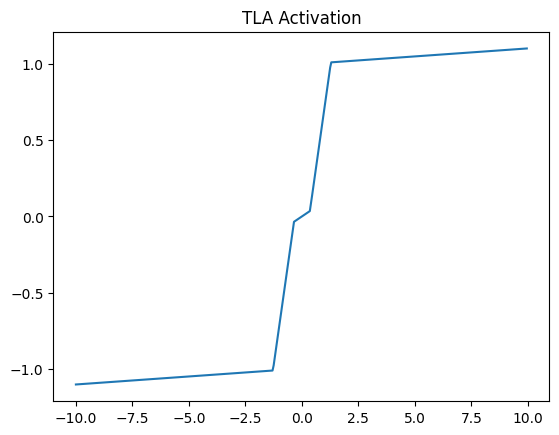
\includegraphics[width=0.35\textwidth]{tlaAct.png}
    \caption{the proposed activation function}
\end{figure}

The proposed function is a simple piecewise linear approximation of a sigmoid or tanh pattern activation function, with a guaranteed minimum gradient at its extrema. This minimum gradient is left as a parameter that can be adjusted by the user. At lower values, this function closely approximates a hard threshold, but will experience vanishing gradients. At higher values,  the minimum gradient increases, but the thresholding capability is lost.

\subsubsection{Validating the principled approach}
In order to provide a demonstration of the practical utility of our general theoretical observations for time series modelling with deep models, we demonstrate a model for R peak classification that takes these observations into account. We compare this against the results of a more traditional unprincipled model that is structurally similar to the current state of the art deep models for ECG analysis.

All training was done on batched data, with batches consisting of two adjacent samples of an ECG signal. The exact details of each architecture are shown in Appendix A.


\paragraph{\textbf{Conventional ResNET Deep Learning Model}}
As a baseline, we implemented a 1 dimensional Residual CNN model, based on \cite{stanfordML}. This reflects the current state of the art for ECG analysis.


\paragraph{\textbf{Wavelet ResNET Deep Learning Model}}
As a demonstration of principled model design, we propose a deep learning architecture that should, while similar in nature to the prior model, generate predictions that are more robust to local variations in the noise and R peak amplitudes. This model will consist of a residual CNN model, with a few key differences to that mentioned previously.

By our above discussion, in a traditionally architected and optimised deep model, this is inherently impossible to achieve while still being trainable. 

The proposed architecture, and the basis for the choice of each component is as follows:

\begin{enumerate}
    \item The model will incorporate an auto-encoder style model, with a block of convolutional operations followed by a block of de-convolutional on the data
    \item To better preserve shift invariance, this model uses dilated filters rather than pooling to achieve the downsampling effect in the autoencoder
    \item The ReLU activations are replaced with our proposed activation above that attempts to trade-off  trainability and thresholding capability, based on the choice of hyper-parameter
\end{enumerate}

\paragraph{\textbf{Wavelet Based Deep Learning Model}}

We will also implement a much more aggressively simplified deep CNN model that almost identically resembles the structure of a wavelet transform.

This is based partially on the implementation from \cite{despawn}. This is similar to the previous model, with the main differences being

\begin{enumerate}
    \item The elimination of BatchNorm and Dropout
    \item The limitation to a single filter per CNN layer
    \item The use of pooling rather than dilation to correspond to a true wavelet (rather than  à trous) transform
\end{enumerate}

We also fitted a derivative of this model, where, the re-composition filters were not learnable, but acted as the quadrature mirror filters for their corresponding decomposition filters (computed by reversing the decomposition filter and flipping the signs of alternate elements), as per \cite{despawn}.

The fitting of models b) and c) above requires more hyper-parameter optimisation, particularly around the choice of minimum gradients in the activation functions.

For this reason, a series of lower-complexity wavelet models were fitted on the data, and cross-validated metrics were used to identify the appropriate sets of hyper-parameters to develop a model of similar scale to the conventional ResNET.

\subsubsection{Model Summaries}

All models were fitted with homogeneous batches of 2 ECG samples of length 4096 signals (sampled at 360Hz). Models were trained with 10 fold cross validation (folds are randomised between models), for 50 epochs per fold. Input data were normalised for all models. Model losses were computed as binary corssentropy to the true 1/0 R peak positional series.

Kernel sizes were held at 16 for simplicity, and allow for fairer comparability between models. 64*(block index) kernels were fit for each convolutional operation in each block for the standard ResNET. 8 kernels were similarly fit in the Wavelet style model. The pure wavelet model fit a single kernel per convolutional layer. 

\begin{center}
    \begin{tabular}{ |p{3cm}||p{3cm}|p{3cm}|p{3cm}|  }
     \hline
     \multicolumn{4}{|c|}{Table 1: Details of fitted models} \\
     \hline
     Model Class& Residual Blocks/Decomposition Levels & Activation Gradient Parameter & No. Trainable Parameters \\
     \hline
     \multirow{4}{4em}{Standard ResNET}  & 1   & - & 198\,272 \\
                                        &   2  & -& 723\,328   \\
                                        & 3 & -& 2\,100\,672\\
                                        & 5 & - & 8\,985\,088\\ 
      \hline
      \multirow{6}{4em}{Compact Wavelet Style ResNET}  
                                        & 3 &  0.01 & 21\,041\\
                                        & 5 & 0.01 & 90\,475 \\
                                        & 3 &  0.05 & 21\,041 \\
                                        & 5 & 0.05 & 90\,475\\
                                        & 3 & 0.5 & 21\,041 \\
                                        & 5 & 0.5 & 90\,475\\
        \hline
        \multirow{9}{4em}{Traditional Wavelet}  
                                        & 2 &  0.01 & 133\\
                                        & 5 & 0.01 & 328 \\
                                        & 7 &  0.01 & 458 \\
                                        & 2 &  0.05 & 133\\
                                        & 5 & 0.05 & 328 \\
                                        & 7 &  0.05 & 458 \\
                                        & 2 &  0.1 & 133\\
                                        & 5 & 0.1 & 328 \\
                                        & 7 &  0.1 & 458 \\
                                     
        \hline

        \multirow{5}{4em}{Shared QMF}  
                                        & 2 &  0.01 & 37\\
                                        & 2 &  0.05 & 37\\
                                        & 2 &  0.075 & 37\\
                                        & 5 & 0.01 & 88 \\
                                        & 5 & 0.05 & 88 \\                          
                                     
        \hline
    
    \end{tabular}
\end{center}


\subsection{Empirical Experiment Results}

The first and most obvious comparisons to make between models are between the cross validated prediction losses.

\begin{figure}[H]
    \centering
    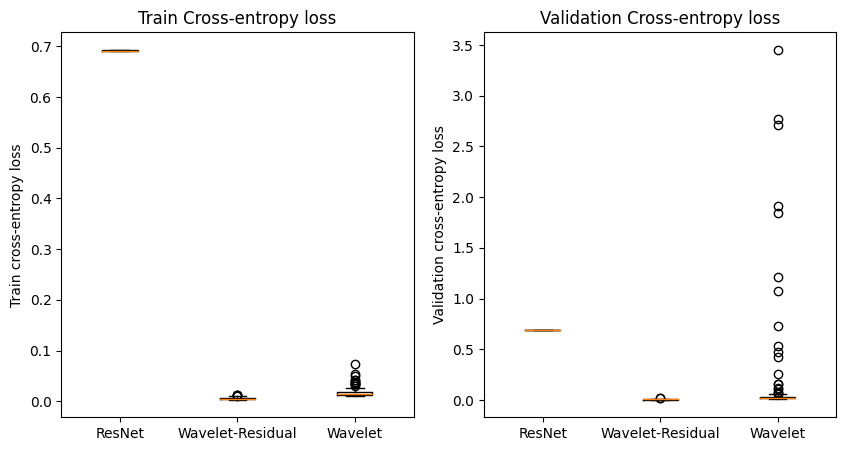
\includegraphics[width=0.5\textwidth]{full_loss.png}
    \caption{Cross validated Cross-entropy loss on the models in Table 1}
\end{figure}

\begin{figure}[H]
    \centering
    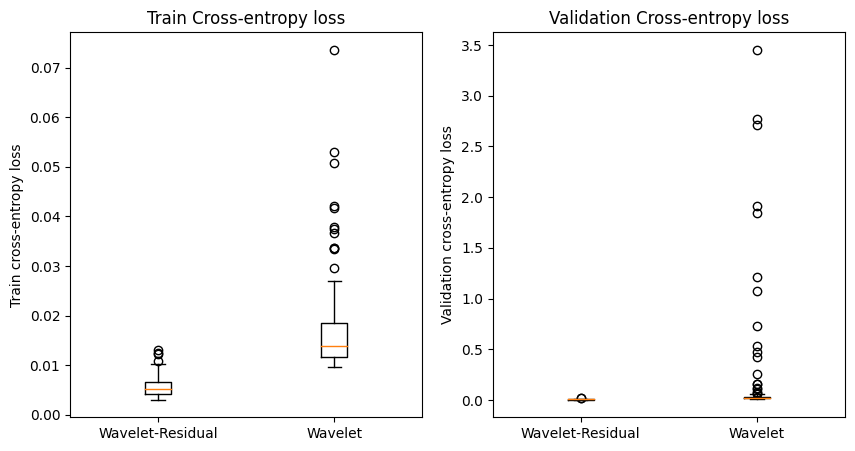
\includegraphics[width=0.5\textwidth]{full_wavelet_loss.png}
    \caption{A clearer view of the differences between the predictions on the wavelet based models in Fig 3.}
\end{figure}

While initial indications are that the wavelet models vastly outperform the ResNET model, even though they involve vastly fewer parameters, the situation is more nuanced.

Before this can be addressed, we must first account for the greater variability between the wavelet based models than the ResNET models. This is to be expected, since the hyperparameters were more varied over these models - it is therefore appropriate here to select a well performing set of hyper-parameters, and proceed to perform further comparisons with this limited set of models. This should result in fairer and more appropriate comparisons between model classes.

To do this, we will consider the cross-validated prediction losses of the models within each class, and select representative well-performing subsets of each class accordingly.


\begin{figure}[H]
    \centering
    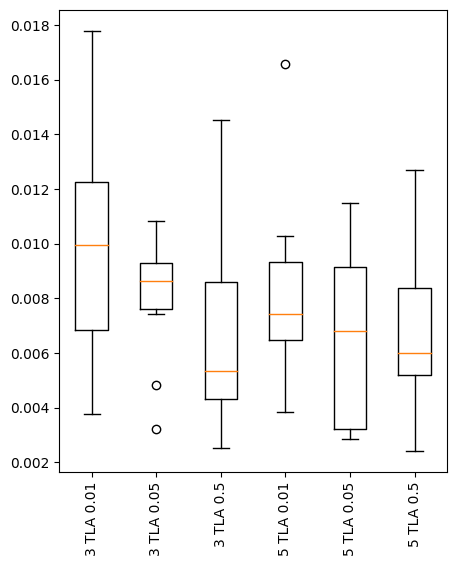
\includegraphics[width=0.2\textwidth]{waveletStlyeParams.png}
    \caption{Overall validation losses for wavelet based ResNET implementations}
\end{figure}

\begin{figure}
    \centering
    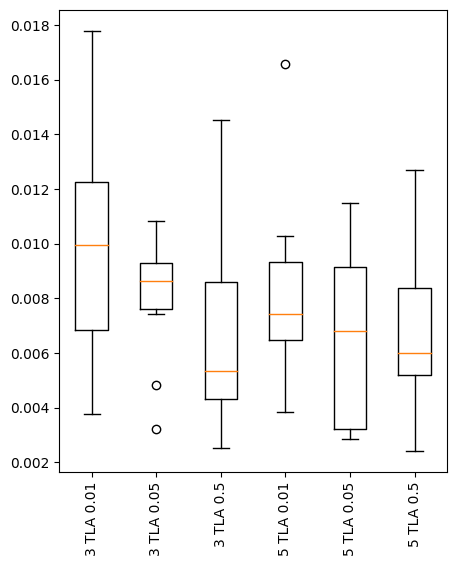
\includegraphics[width=0.2\textwidth]{waveletStlyeParams.png}
    \caption{Overall validation losses for standard ResNET implementations}
\end{figure}


\begin{figure}
    \centering
    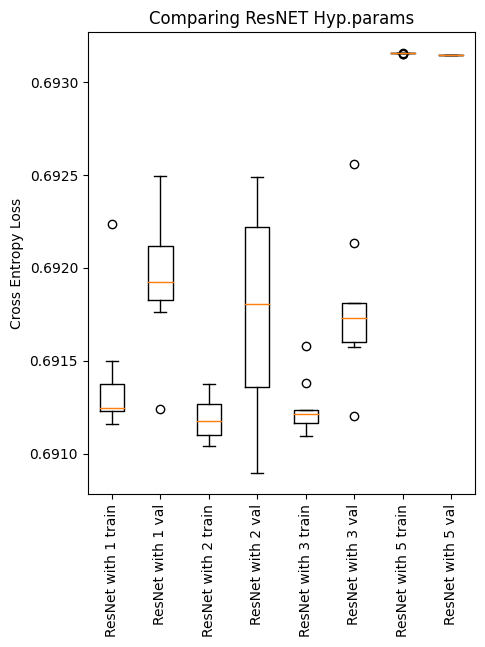
\includegraphics[width=0.35\textwidth]{resnetParams.png}
    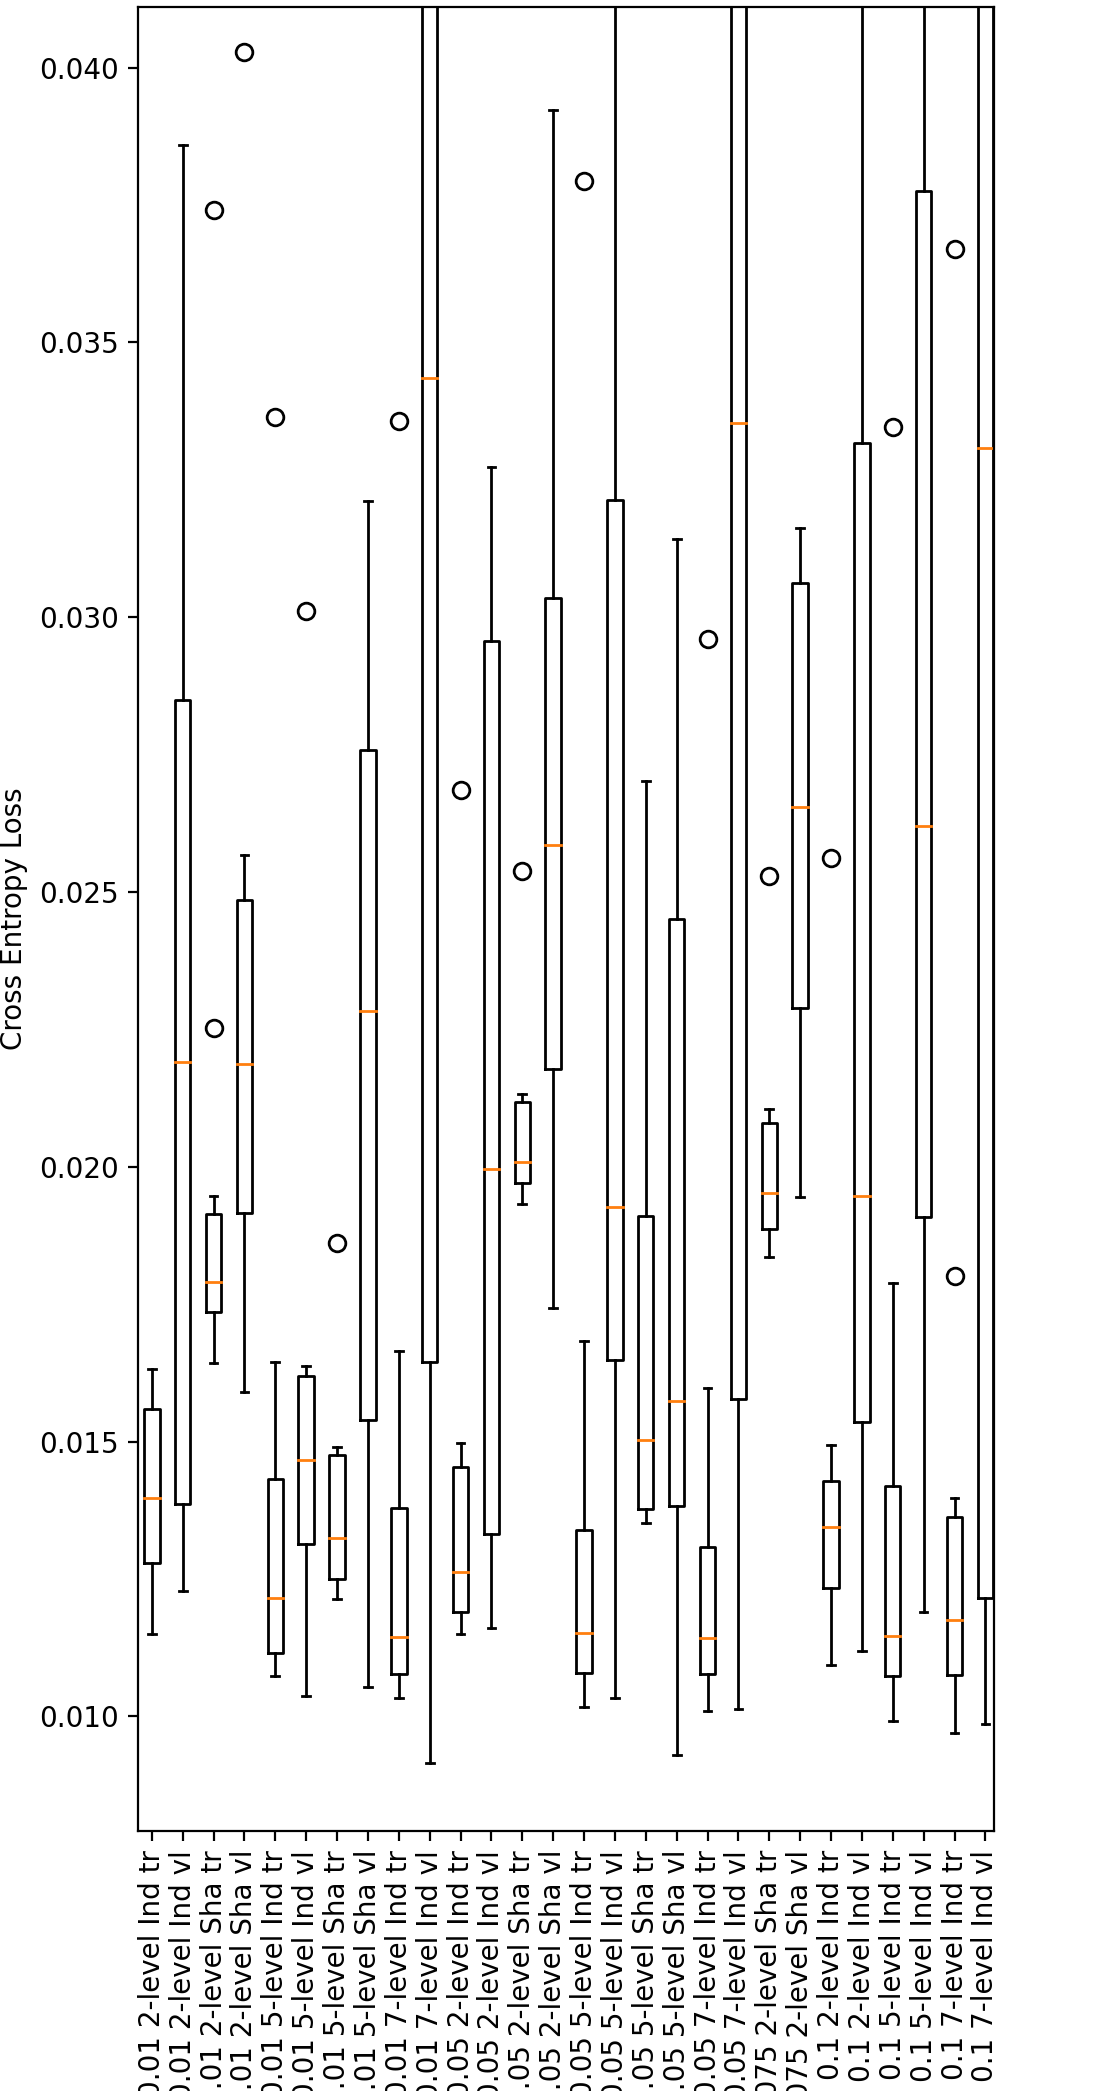
\includegraphics[width=0.35\textwidth]{waveletParamLossesDetail.png}
    \caption{Overall validation losses for simple wavelet implementations. (Zoomed detail on right)}
\end{figure}

\clearpage


\subsubsection{Model Selection}

We do not take a rigorous and exacting model selection approach here to find the definitive highest performance by some metric. The reason for this is two-fold:

\begin{enumerate}
    \item We wish to avoid overly overfitting to random variation in the validation losses
    \item The exact losses of our final model are not the important aspect of this experiment - the general performance differences between the different classes are what interests us here. The performance differences of typical, not necessarily optimally parameterised, models suffice to explore these differences between model classes
\end{enumerate}

As a general observation on the plots, models with 5 wavelet coefficients and an activation gradient parameter of 0.05 achieve consistently low losses, albeit not necessarily the absolute lowest in each model class. Based on this observation, further evaluation of results will be restricted to the models listed in Table 2.

\begin{center}
    \begin{tabular}{ |p{3cm}||p{3cm}|p{3cm}|p{3cm}|  }
     \hline
     \multicolumn{4}{|c|}{Table 2: Details of fitted models} \\
     \hline
     Model Class& Residual Blocks/Decomposition Levels & Activation Gradient Parameter & No. Trainable Parameters \\
     \hline
        \multirow{2}{4em}{Standard ResNET}  
                                        &   2  & -& 723\,328   \\
                                        & 3 & -& 2\,100\,672\\
      \hline
      \multirow{2}{6em}{Wavelet Style ResNET}  
                                        & 5 & 0.05 & 90\,475 \\
                                        & & & \\
        \hline  
    \multirow{2}{6em}{Wavelet Style ResNET}  
                                        & 5 (32*layer index kernels per layer) & 0.05 & 1\,406\,299 \\
                                         & & & \\
        \hline
     \multirow{3}{7em}{ResNET-Wavelet, Non-QMF}  
                                    & 5 & 0.05 & 328 \\
                                     & 5 & 0.01 & 328 \\ & & & \\
    \hline

    \multirow{3}{6em}{Traditional Wavelet - QMF Filters}  
                                    & 5 & 0.05 & 88 \\
                                     & 5 & 0.01 & 88 \\
                                     & & & \\
    \hline
    \end{tabular}
\end{center}



\subsubsection{Comparing Losses on the R peaks and non-R peaks}



\begin{figure}[H]
    \centering
    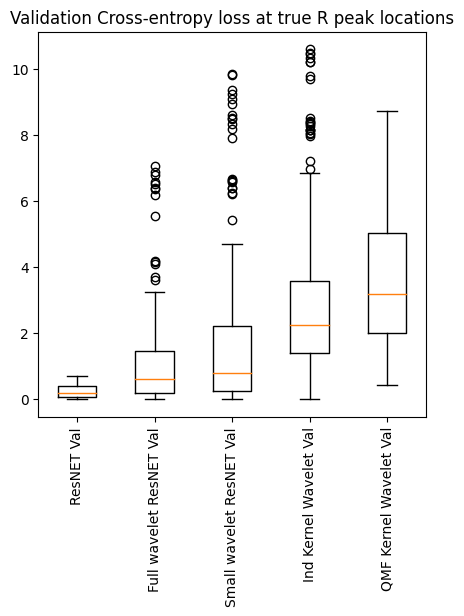
\includegraphics[width=0.3\textwidth]{valLossAtRBoxplots.png}
    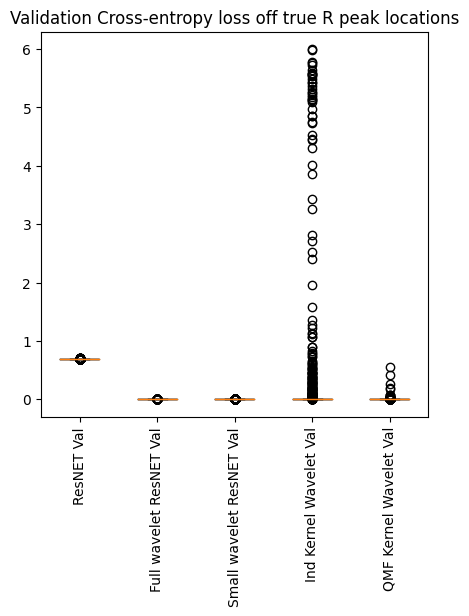
\includegraphics[width=0.3\textwidth]{valLossOffRBoxplots.png}
    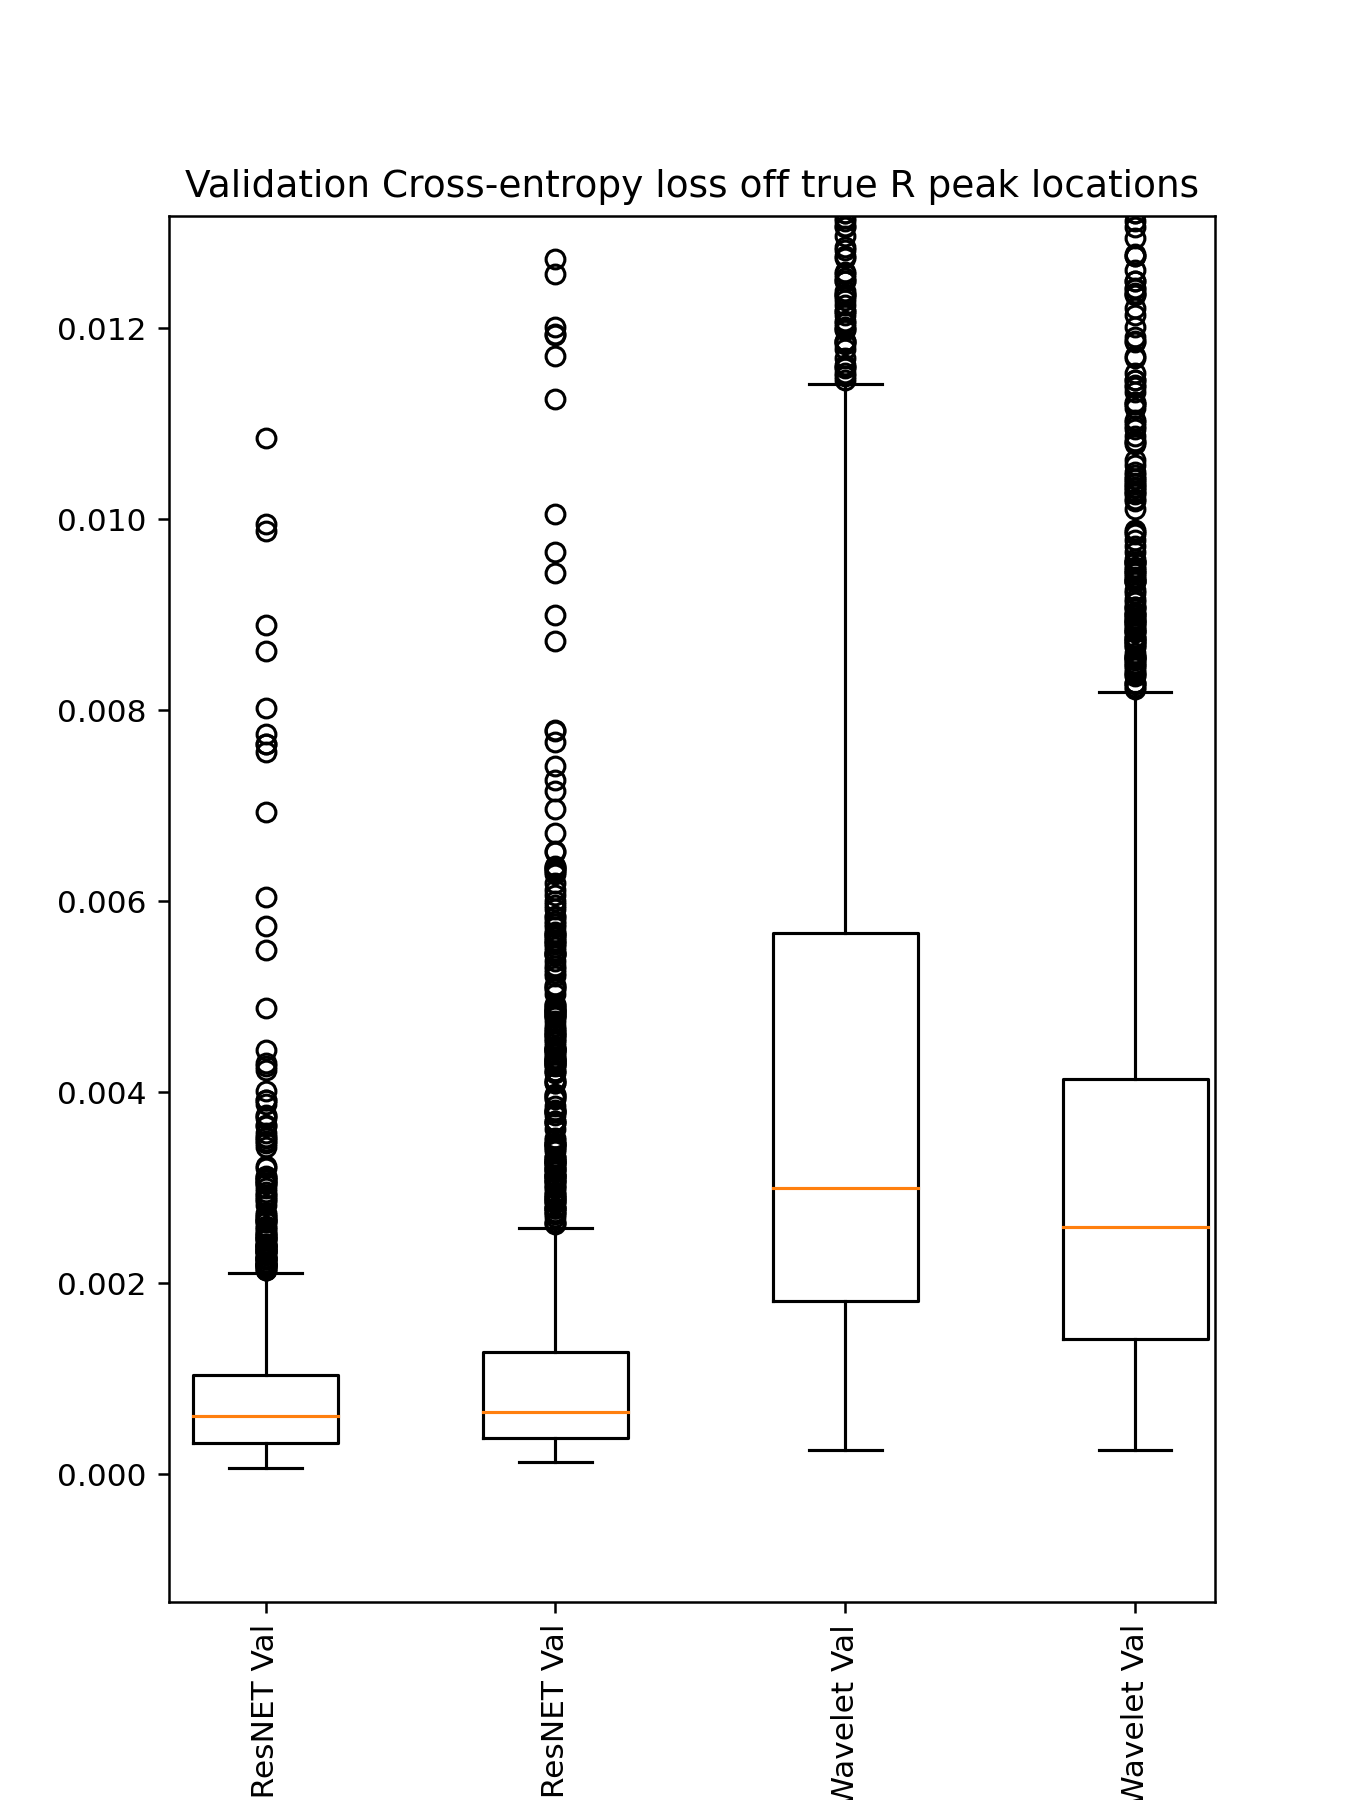
\includegraphics[width=0.3\textwidth]{valLossOffRBoxplotsZoomed.png}
    \caption{Validation loss at R peak and non-R peak points. All models correspond to those listed in. Rightmost plot is a zoomed section of the centre plot that better illustrates the differences between the last 4 boxes.}
\end{figure}



Interestingly, separating the loss into the components of loss incurred by true positives and true negatives serves to better differentiate the performances of the different models. 

The first immediate observation here is that the prediction loss declines for the less sophisticated wavelet based models. For this reason, we will initially consider only the differences in performance between the standard and wavelet style ResNET/residual models. We will revisit the other wavelet models in a further section.

\paragraph{\textbf{Comparing Performance Between Standard and Wavelet ResNET}}
In the plots of the cross validated losses for the standard and wavelet ResNET, we see that the validation losses are lower for the standard model when considered solely on the true R peaks, and lower for the wavelet model on the other portions of the input signals. Both of these differences are found to be statistically significant by a Mann-Whitney U test (R peak validation losses are significantly lower for the wavelet ResNET, non-R peak validation losses are significantly lower for the standard ResNET) at $p=0.05$ level of significance.

Further Man-Whitney U tests also indicated that 

\begin{enumerate}
    \item Mean R peak \textit{prediction values} (\textbf{not losses}) are significantly lower for the standard ResNET
    \item Mean non-R peak \textit{prediction values} are significantly lower for the wavelet ResNET
\end{enumerate} 

This can be easily visualised by examining the distributions of the cross-validated prediction values for the different model classes.

\begin{figure}[H]
    \centering
    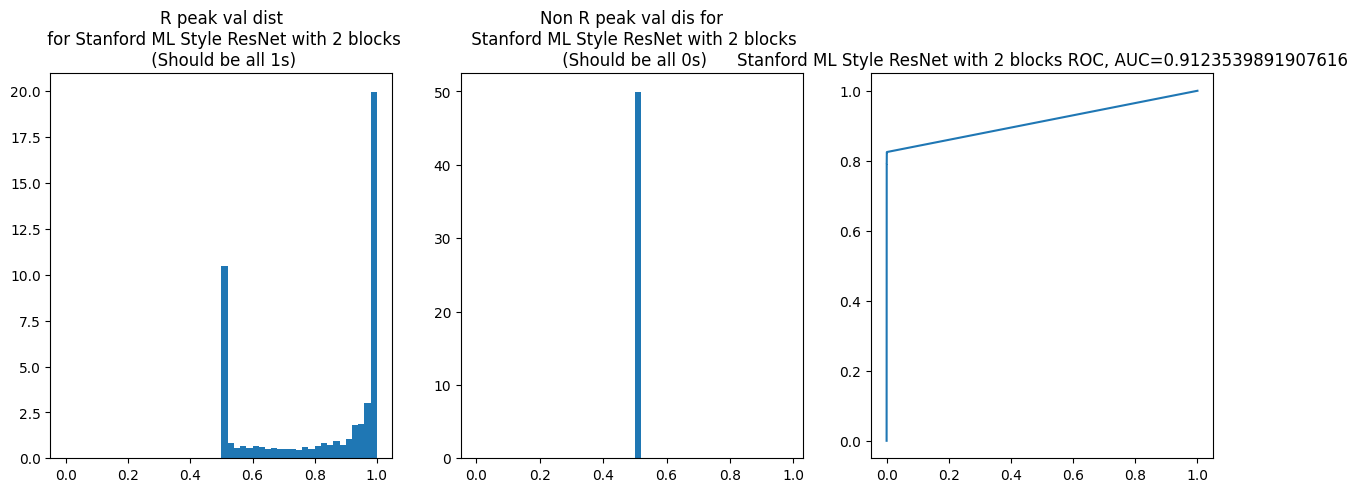
\includegraphics[width=0.75\textwidth]{resnet2Dist.png}
    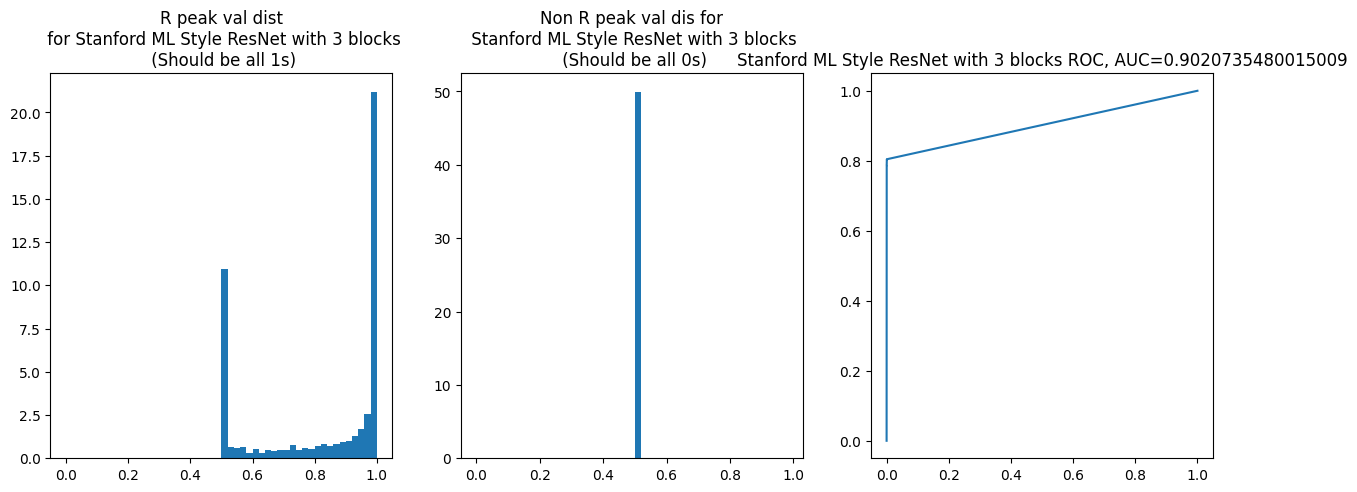
\includegraphics[width=0.75\textwidth]{resnet3Dist.png}
    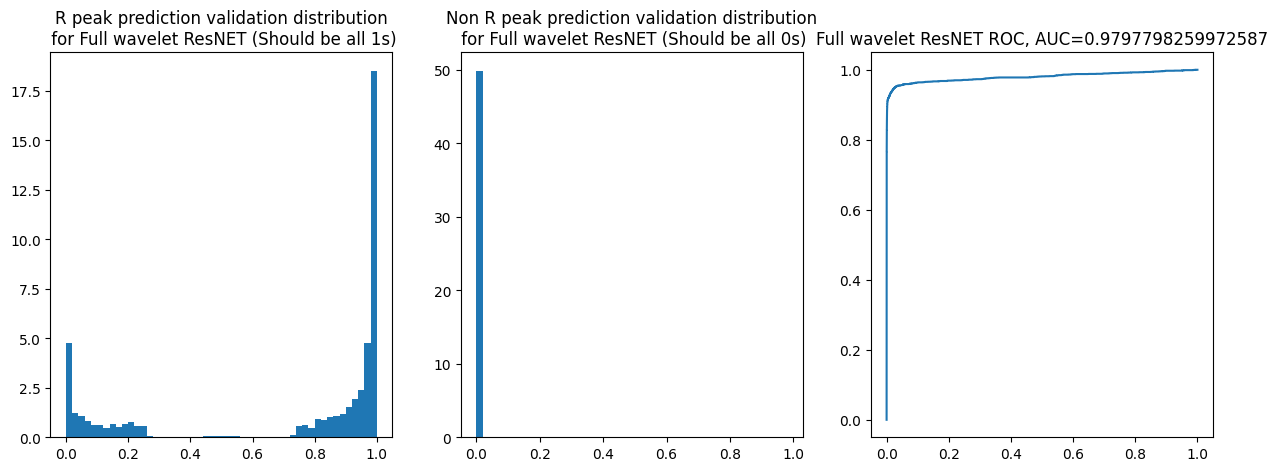
\includegraphics[width=0.75\textwidth]{waveletNetDist.png}
    \caption{Cross-validated predicted values for indicated models.}
\end{figure}

The most glaring difference here is that the standard ResNET model predictions have a lower bound of 0.5 rather than 0. This provides an obvious limitation for predictive accuracy.

Clearly, the Wavelet ResNET model is much more successful at separating the 0 and 1 predictions. Now, let us superimpose the predictions for the 3 block standard ResNET and the 5 layer (32*(block index)  kernel per block) wavelet ResNET model. These models consist of ~2M and ~1.4M trainable parameters respectively, and are thus of a similar order of complexity.

\begin{figure}[H]
    \centering
    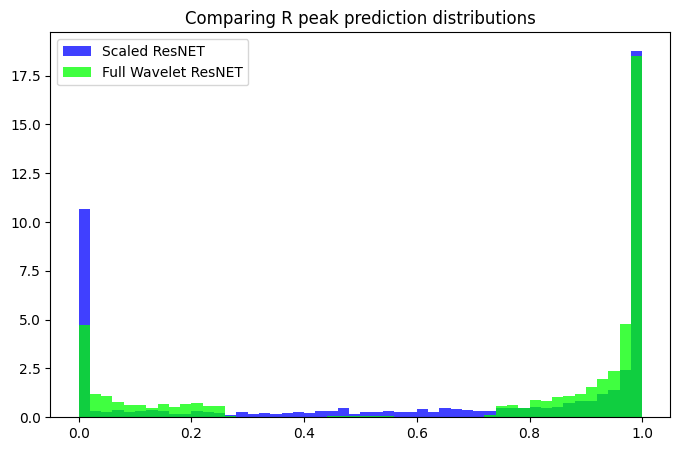
\includegraphics[width=0.45\textwidth]{compRESNETWAVELET.png}
    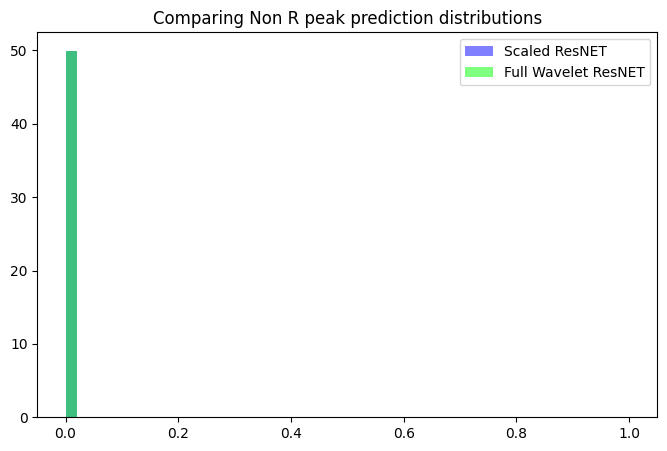
\includegraphics[width=0.45\textwidth]{compRESNETWAVELET_nonr.png}
    \caption{Manually adjusting standard ResNET predictions, and overlaying wavelet ResNET predictions.}
\end{figure}

Even when the standard ResNET outputs are manually normalised to be more favourable, we see that the wavelet ResNET model has more robust performance.

Based on a 95\% bootstrap CI, we can observe that between (26\%,29\%) of cross validated predictions from a wavelet ResNET model are less than 0.5

In contrast, the same interval computed on the standard ResNET gives (33\%,36\%). Therefore, we can conclude that the wavelet is significantly better at correctly identifying R peaks, \textbf{even when the standard wavelet outputs are manually normalised}.

We also see that there is a clearer visual separation of the wavelet ResNET predictions on the true R peaks. The predictions on the rest of the signals coincide almost perfectly for both models. While ideally the models should be predicting all 1 values for the validation R peaks, this is potentially a positive indication that the wavelet model has intrinsically higher capability to form a clearer decision boundary.

It is worth again noting that this wavelet model contained ~1.4M trainable parameters, to the standard model's ~2M - highly suggestive that the wavelet structure is an inherently more stable and accurate architecture for this specific problem. We suspect under a further simplified the Wavelet ResNET, the performance will remain competitive with the higher complexity standard ResNET, however further research is required to verify this hypothesis.

Appendix B contains sample train and validation predictions from both standard ResNET and Wavelet ResNET models. While \textbf{not} a useful or reliable indicator in themselves, they serve to visually represent our results above in context - the predictions from the Wavelet model \textit{appear} more consistent, robust and well separated.

\paragraph{\textbf{Comparing Simpler Wavelet Models}}

\begin{figure}[H]
    \centering
    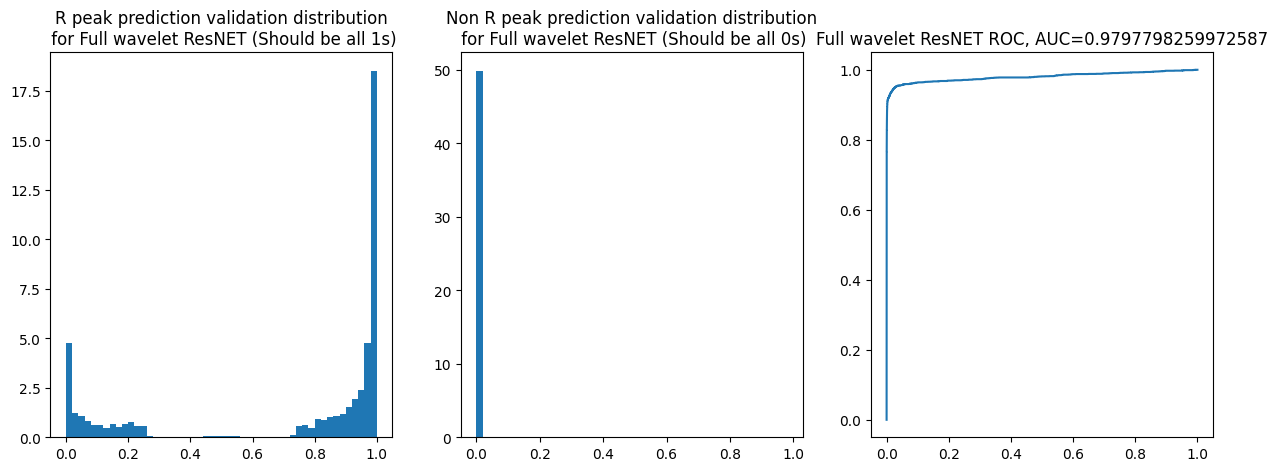
\includegraphics[width=0.75\textwidth]{waveletNetDist.png}
    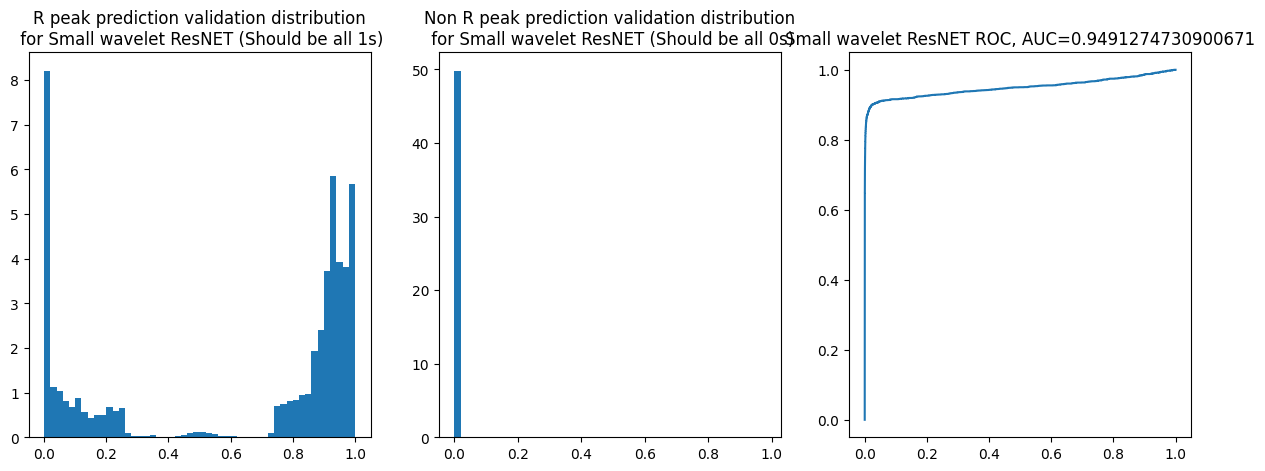
\includegraphics[width=0.75\textwidth]{smallWaveletNetDist.png}
    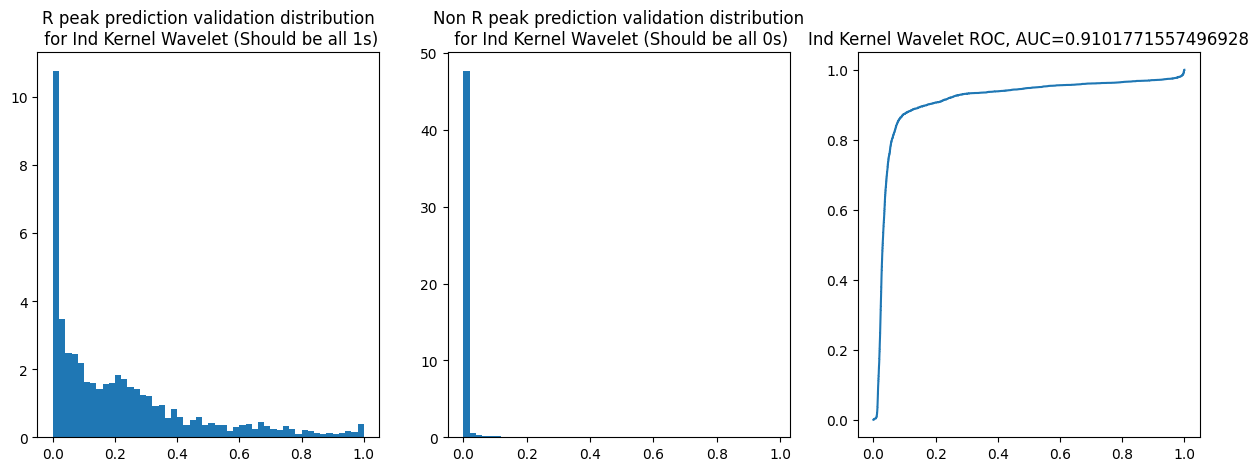
\includegraphics[width=0.75\textwidth]{indWaveletDist.png}
    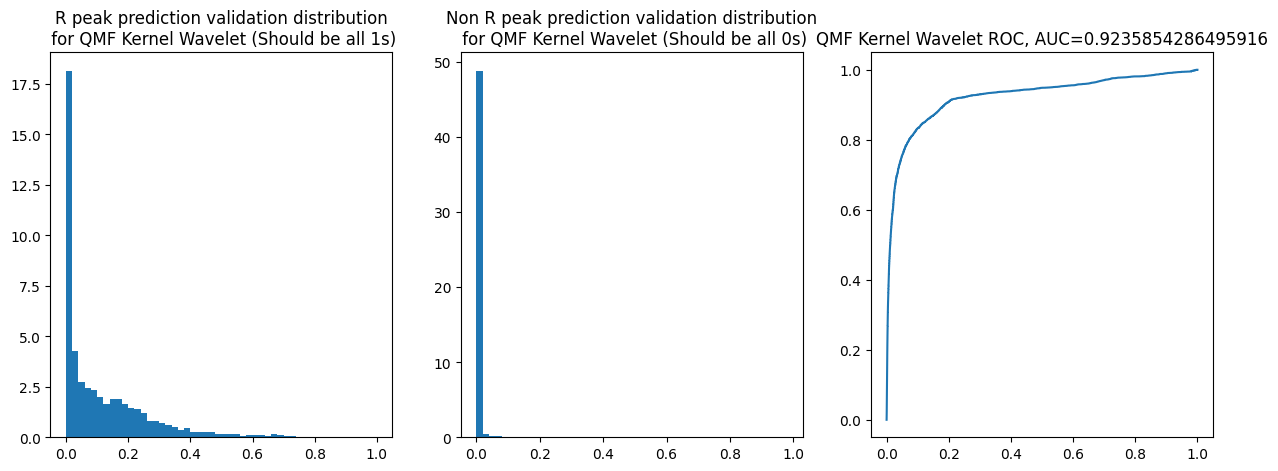
\includegraphics[width=0.75\textwidth]{qmfWaveletDist.png}
    \caption{Cross-validated predicted values for indicated models.}
\end{figure}

While the simple wavelet based models quickly optimised to a lower loss value, their predictions have a clear right skew - the exact opposite of what is desirable. These simple wavelet models are likely struggling to achieve the conditionally independent outputs. This is due to the intrinsic lack of ability of these models to achieve trainability and construction of a decision boundary equivalent to the threshold operations in a pure wavelet decomposition.

As a result, we expect that the more complex models (such as the wavelet style ResNET) are needed to heavily pre-process the data to achieve the most favourable results with largely static decision boundaries.

The fact that the validation losses of these models are lower than the standard ResNET model is notable in this case, considering that the smallest of these models are a \textbf{factor} of approximately 20\,000 times smaller than the ResNET model. This is strongly indicative that it is likely fruitful to conduct a dedicated study on the optimisation of such small wavelet models on this data.

There are a number of potential directions which could be explored to develop such models

\begin{enumerate}
    \item Considering the use of algorithme à trous rather than pooling based downsampling
    \item Iteratively reducing the gradient parameters of the novel activation functions as training progress, gradients converge and learning gradually slows. This would lead to learnable models that \textbf{converge to} effective threshold operations/decision boundaries
    \item The benefits of using hyper-parametric kernel filters that correspond to known band-pass filters that are generally optimal in standard wavelet transforms
    \item Potential benefits of having multiple such filters in each layer acting in parallel. When combined with dropout, this could correspond directly to bagged predictions, which could be more robust, while only linearly increasing the  number of coefficients in the model
\end{enumerate}

\section{Discussion \& Conclusions}

\begin{enumerate}
    \item We have considered an arbitrary neural network layer that attempts to learn a decision threshold, above and below which it is conditionally independent of variations in the data. We have shown that such a layer cannot both fully respect this property, and be gradient-optimisable. The choice of activation function is what dictates this tradeoff, with a negative linear relationship between the lower-limit on the gradient of the activation function, and the degree of its unboundedness
    \item We have shown how this problem extends to multi-layer neural networks
    \item We have demonstrated that batch normalisation corresponds to the construction of an \textit{adaptive threshold} for this decision boundary, and that it does not eliminate or negate the above issue
    \item We have proposed a general form of piecewise activation function that allows for the manual tuning of this trade-off
    \item We have explored the similarity between dilated connections in CNN models and the algorithme à trous, and noted how these lead to more robustly shift invariant layers
    \item We have described ECG signals in terms of their characteristics as a time series. We considered the specific clinical problem of automated R peak extraction, and descried this as a general time series problem. In particular, we focused on the conditional invariance of the outputs, which are purely positional in nature, to local amplitude variations in the input data. This makes the aforementioned theoretical principles that we derived critical for model design
    \item We broadly demonstrated, that taking a principled approach to CNN model design, involving the creation of models that are more cognisant of the above theoretically-derived principles, leads to models that have more accurate and robust predictions, at potentially lower levels of model complexity. These models are not only more effective at performing R peak extraction, but in fact are likely to produce better results for any stationary, variably periodic time series model that requires localisation of some periodic component, with conditionally amplitude invariant outputs  
    \item This demonstrates that for any practical time series applications, approaching neural network model design by more carefully considering and accounting for respect or violation of known time series properties is potentially highly beneficial
\end{enumerate}

\section{Future Research}

\subsection{Further Empirical Experimentation}
The most obvious continuation of this research would be to perform more experiments to further refine our proposed models to attempt to reach state-of-the art, or close to such performance. This could also be attempted for any arbitrary time series problem in any domain, which exhibits the same characteristics as the problem of R peak extraction.

In the context of ECGs, another avenue of potential research is to attempt to generalise our findings to the multivariate case - such as when we need to extract other temporal components in a conditionally amplitude invariant manner, such as T and S waves. This would require consideration of the most robust way to deal with the relationships \textbf{between} these features, which may require a significant extension of the principles and architectures that we have developed here. From this, there is the possibility to consider the problem of QRS complex detection, and the opportunity to benchmark against the many existing approaches to this problem.

It may also be beneficial to perform a deeper analysis of the efficient design of extreme low-complexity wavelet based CNN models, which have shown good potential in our empirical experimentation.

\subsection{Generalisation to Filter Banks}
It is worth briefly mention in that in general, CNN filters are often to be considered as a form of FIR Matched Filters. These generate a response with an amplitude linked to the presence or non-presence of a template signal (the kernel weights) in an unknown signal. Any threshold or arbitrary decision boundary learned on these outputs that generate predictions will need to exhibit the same conditional amplitude independence as R peak extraction outputs (i.e., are purely positional outputs). As a result, the model experience the limitations that we have discussed here. This may potentially have very widespread consequences for CNN models applied to general time series problems with very minimal sets of assumptions - which could be a serious issue. This warrants further investigation.

\subsection{Non-positional Time Series Characteristics}
By our restriction to the specific issue of conditional amplitude invariance, we have largely neglected to discuss morphological characteristics of signals/time series, and the capabilities of CNNs for such feature extraction.

There are many potential explorations in this area that could lead to powerful, robust models for different classes of problems in a similar vein to our work here. These may include, but are by no means limited to:
\begin{enumerate}
    \item The use of distance measures other than convolution/cross-correlation for Matched Filters
    \begin{itemize}
         \item Dynamic Time Warping filters for problems involving local scaling invariance
         \item Normalised Cross Correlation filters for better amplitude invariance
        \end{itemize}
    \item The potential correspondences between Filter Banks (similar to wavelet decomposition) to CNN architectures
    \item The potential correspondences between clustering algorithms, particularly K-Shape\cite{paparrizos2015k} clustering, and modified CNN architectures
    \item Potential benefits of incorporating frequency-domain methods to CNN architectures (other than wavelet transforms), particularly Hilbert-Huang transforms
    \item The fundamental limitations of CNN models to extract features that correspond to exact temporal intervals
\end{enumerate}

Finally, once multiple such similar studies are completed, an important area of research would be to investigate the interaction of such models - especially how the stacking or linking of such models affects their convergence and performance.

\section{Acknowledgements}
I would like to thank the staff of the University College Cork Schools of Mathematical Sciences and Computer Science for outstanding tuition and support over the course of my degree.

\vspace{0.5cm}

In particular, I'd like to note my thanks to Professor Gregory Provan, without whose endless patience and support this project would never have come close to starting successfully, much less progressing anywhere.

\clearpage

\bibliographystyle{IEEEtran}
\bibliography{references}

\section*{Appendix A: CNN Architectures}

\begin{figure}[H]
    \centering
    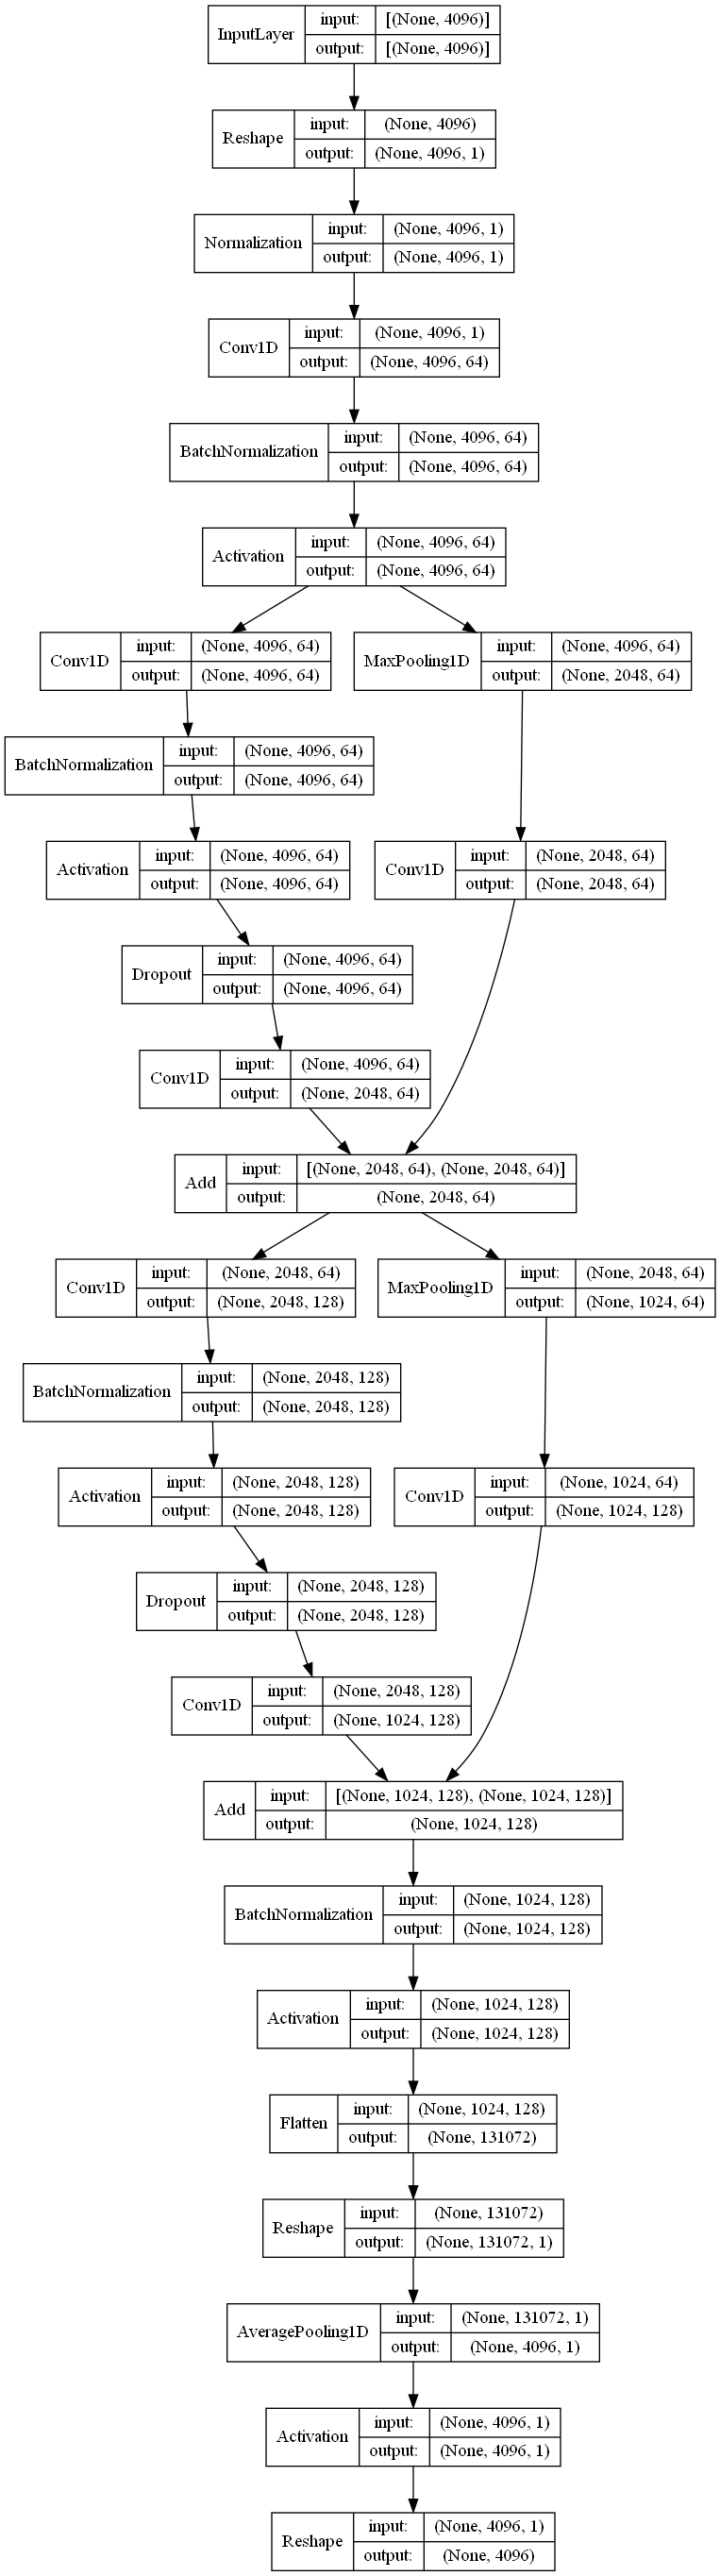
\includegraphics[width=0.35\textwidth]{stanfordmod.png}
    \caption{Conventional Resiudal CNN model, with two residual blocks shown}
\end{figure}

\begin{figure}
    \centering
    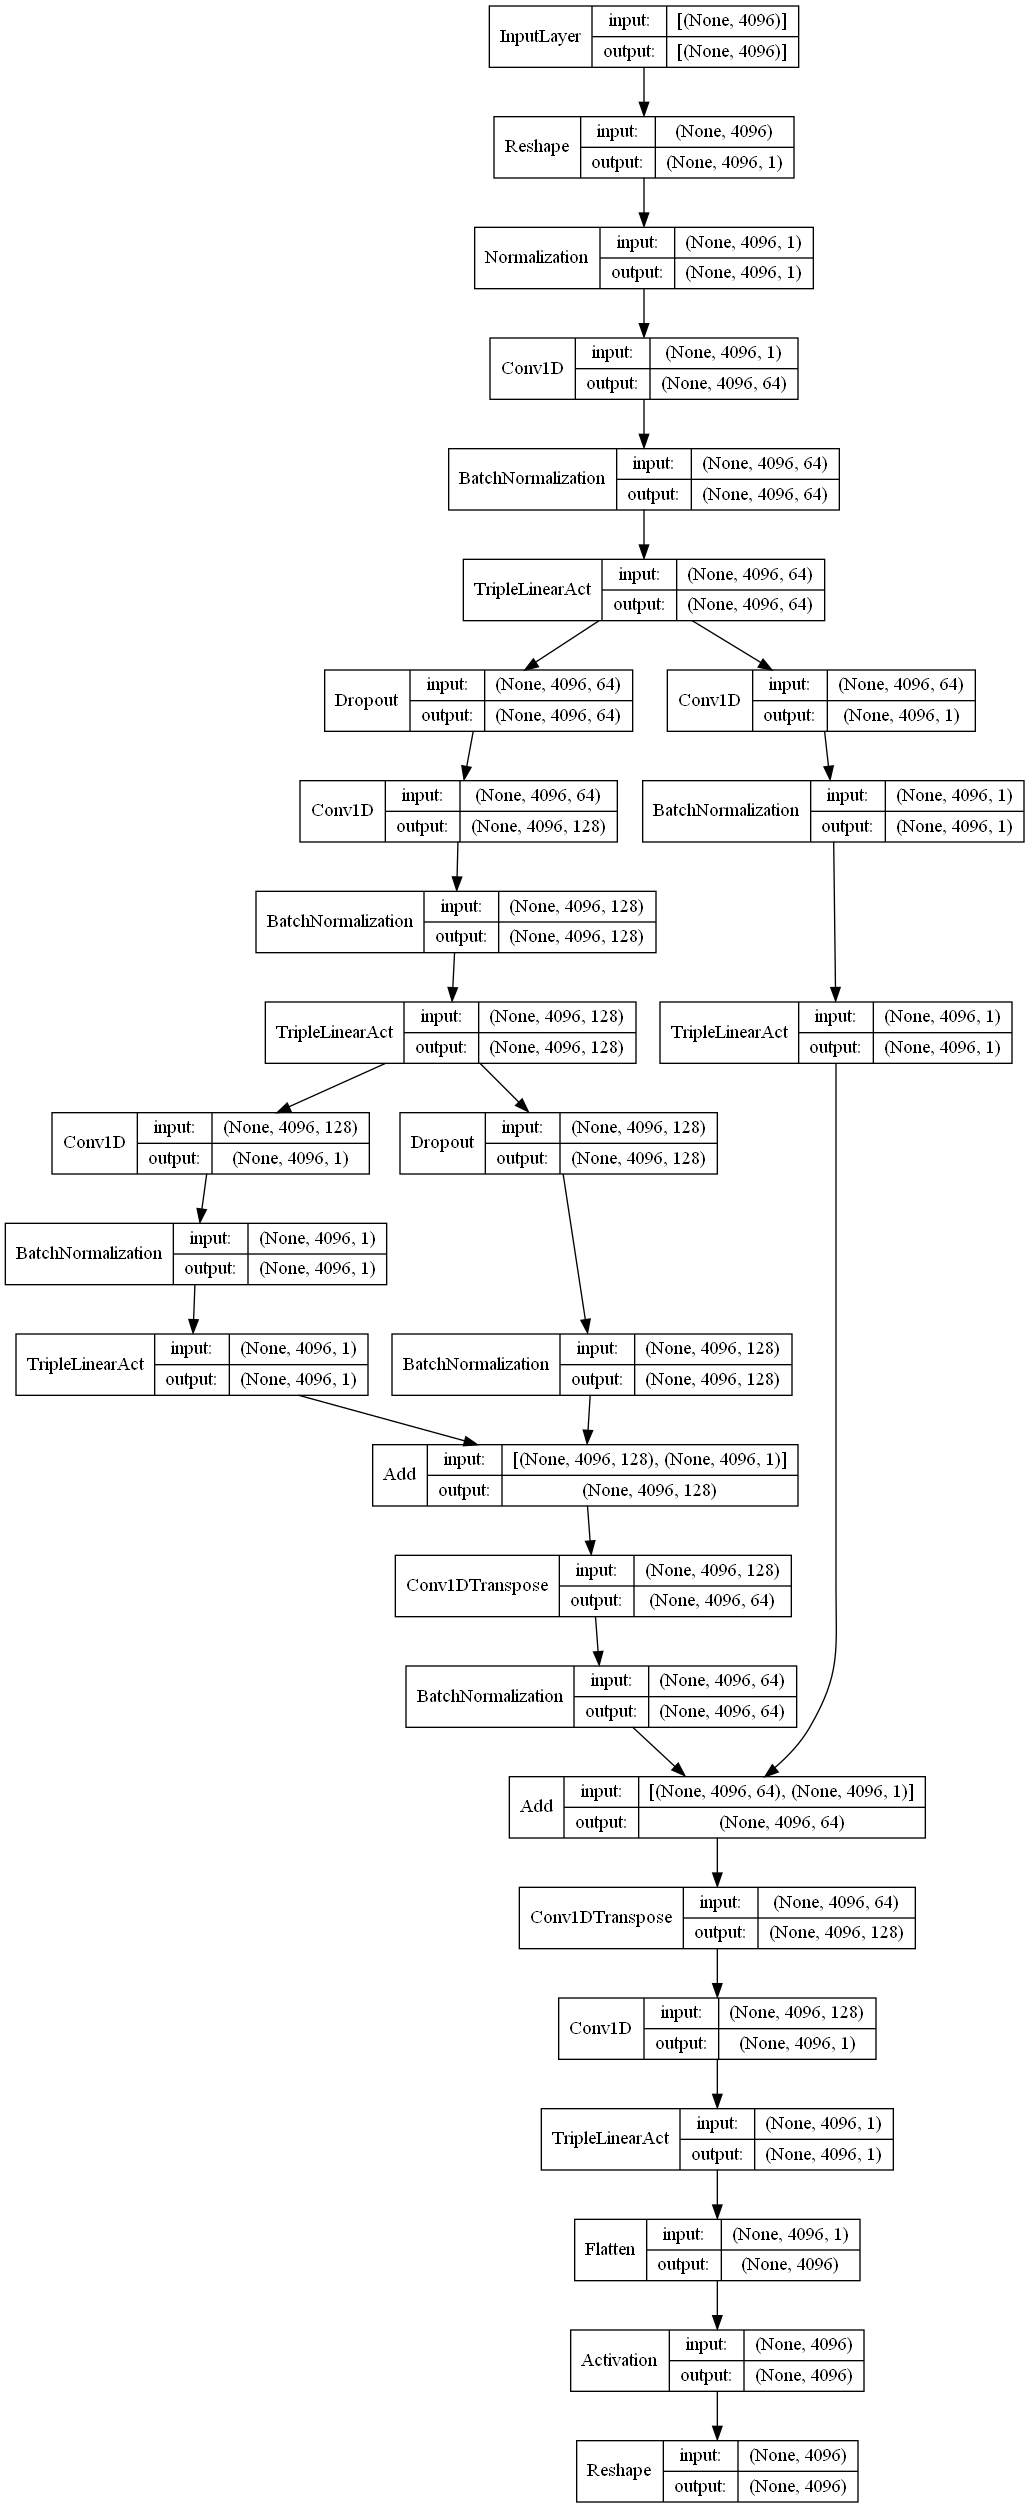
\includegraphics[width=0.5\textwidth]{wavelet_resid.png}
    \caption{Hybrid wavelet-residual CNN model, with two levels of decomposition (and recomposition) shown}
\end{figure}

\clearpage

\section*{Appendix B: Sample Outputs}
Each plot below contains a randomly sampled train and test signal sample, from a randomly chosen cross-validation fold. The samples are different for each model.

\begin{figure}[H]
\centering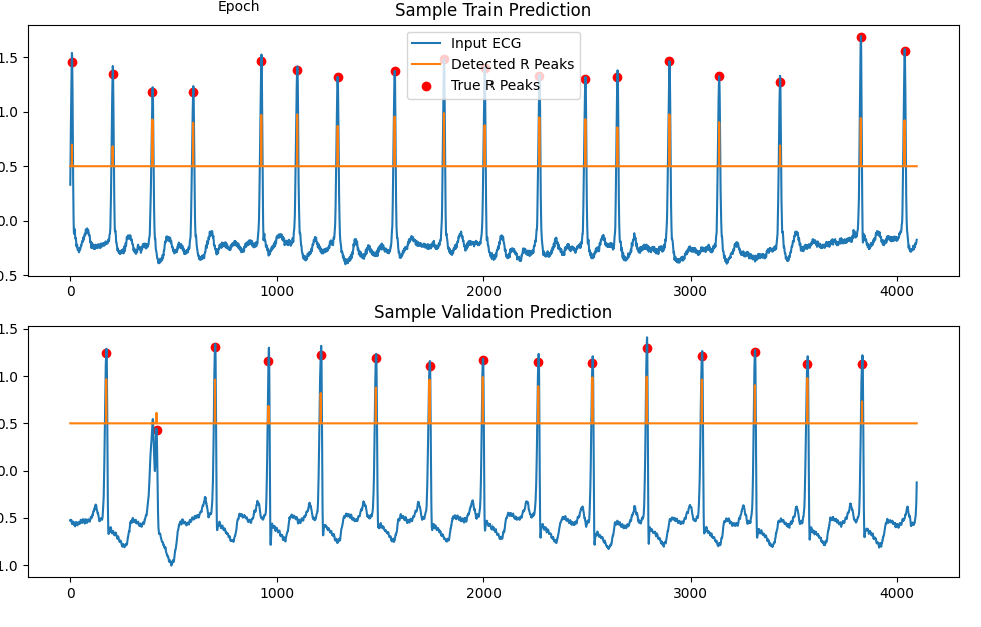
\includegraphics[width = 0.75\textwidth]{resnetPreds.png}
\caption{\label{fig:resNetPreds} Sample outputs of R peak predictions from a standard ResNET model}
\end{figure}

\begin{figure}[H]
\centering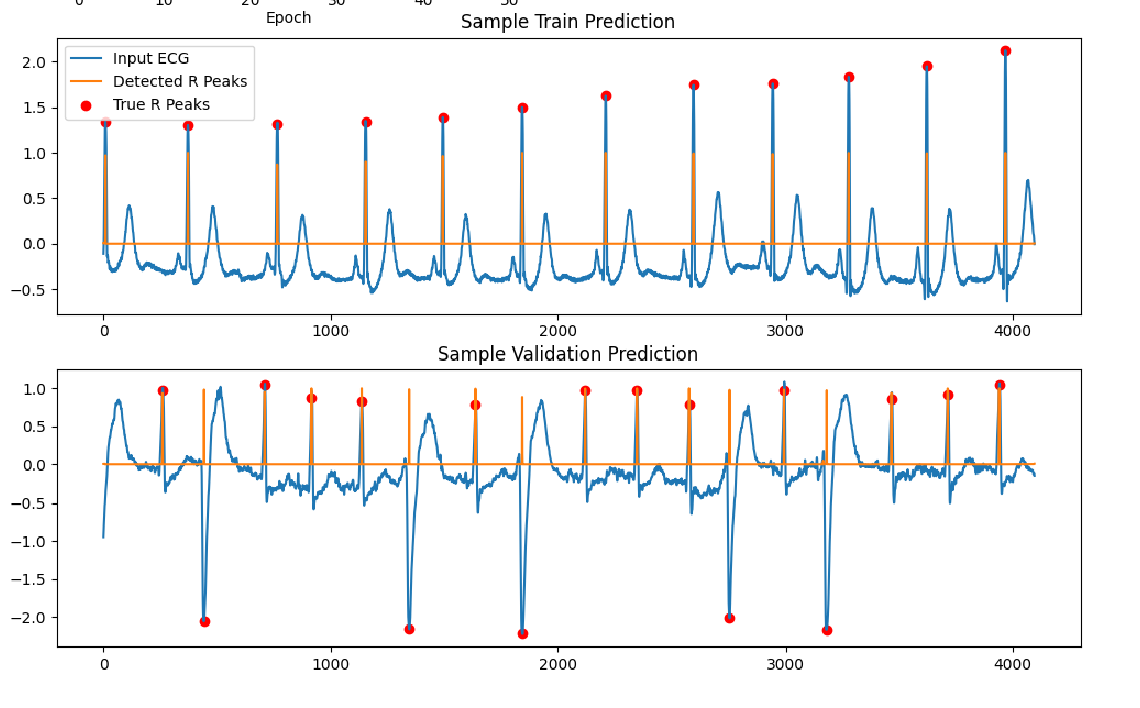
\includegraphics[width = 0.75\textwidth]{waveletFullPred.png}
\caption{\label{fig:waveNetPreds} Sample outputs of R peak predictions from a theoretically motivated Wavelet-ResNET model design}
\end{figure}

\begin{figure}[H]
\centering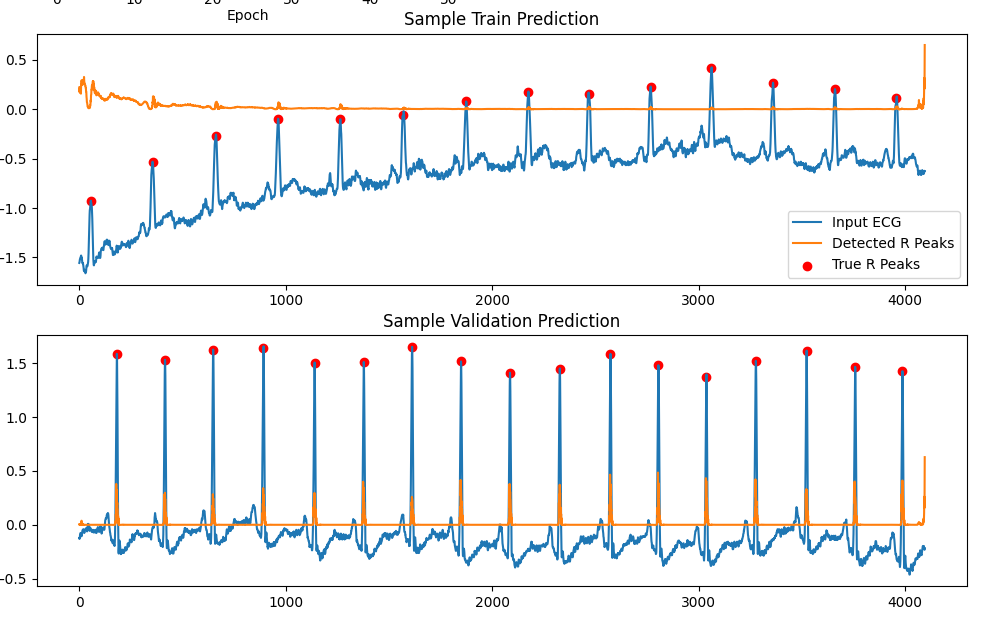
\includegraphics[width = 0.75\textwidth]{qmfPreds.png}
\caption{\label{fig:qmfPreds} Sample outputs of R peak predictions from a wavelet decomposition based model - QMF restricted filters}
\end{figure}

\begin{figure}[H]
\centering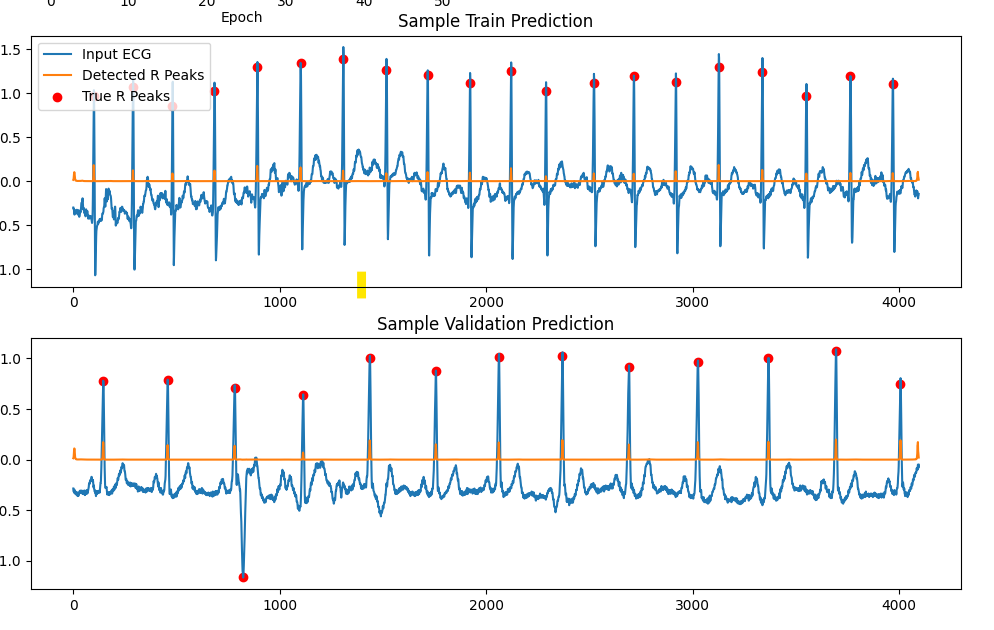
\includegraphics[width = 0.75\textwidth]{indWavelet.png}
\caption{\label{fig:indPreds}  Sample outputs of R peak predictions from a wavelet decomposition based model - urestricted filters}
\end{figure}



\clearpage

\section*{Declaration of Originality}
In signing this declaration, you are conforming, in writing, that the submitted work is entirely your own original work, except where clearly attributed otherwise, and that it has not been submitted partly or wholly for
any other educational award.

I hereby declare that:

\begin{itemize}
    \item This is all my own work, unless clearly indicated otherwise, with full
and proper accreditation;
    \item With respect to my own work: none of it has been submitted at any educational institution contributing in any way to an educational award;
    \item With respect to another’s work: all text, diagrams, code, or ideas, whether verbatim, paraphrased or otherwise modified or adapted, have been duly attributed to the source in a scholarly manner, whether
from books, papers, lecture notes or any other student’s work, whether published or unpublished, electronically or in print.
\end{itemize}

\vspace{5cm}

\begin{tabular}{@{}p{.5in}p{2in}p{.5in}p{2in}@{}}
Signed: & \hrulefill  & Date &  \hrulefill  \\
& Andrew Nash & &\\
& BSc Data Science \& Analytics & &\\
\end{tabular}


\end{document}

